\chapter{Stationary One Body Problem}\label{ch: rotation}

In Chapter \ref{ch:chapter2} we worked the problem of a test particle under the influence of a Schwarzschild gravitational field, means a spherically symmetric and static body. Now we will consider the same test particle but under the influence of a weak gravitational field, generated by a slowly rotating source. \\

The first step to develop this problem is to understand, in a general way, the Kerr metric and Weyl Levi Civita metric \cite{Raine, Frolov, johnandcoulter, erezandrosen}.

\section{Metric of slowly rotating spheroid}

\subsection{Kerr metric}

The Kerr solution is the exact solution of the Einstein field equations; outside a stationary body. In the proper reference frame with no time dependence; Kerr metric, just as the Schwarzschild metric, tends to the Lorentz frame at infinity, i.e., the field is asymptotically ($r \rightarrow \infty$) flat \cite{Brumberg,  Frolov, Raine}.\\

Boyer - Lindquist coordinates $(t,r,\theta, \phi)$ give the asymptotically behavior, using these coordinates, usually called ``Schwarzschild-Like'' coordinates,

\begin{align}
\begin{split}
	ds^2 = -\frac{\Delta - a^2\sin^2\theta}{\rho^2} dt^2 +\frac{4ma}{\rho^2} r \sin^2\theta d\phi dt +\frac{\rho^2}{\Delta}dr^2 + \rho^2 d\theta^2 + \frac{A\sin^2\theta}{\rho^2}d\phi^2
	\label{eq: kerrmetric}
\end{split}
\end{align}
\begin{subequations}
\begin{align}
	&\Delta = r^2 - 2mr +a^2\\
	&\rho^2 = r^2 + a^2\cos^2\theta\\
	\label{eq: Ag33}
	&A = (r^2+a^2)^2 - a^2\Delta \sin^2\theta.
\end{align}
\end{subequations}

The metric depends on two parameters $m$ and $a$. At large distances, $r \rightarrow \infty$, the metric given in (\ref{eq: kerrmetric}) is

\begin{align}
	ds^2 = -\left(1-\frac{2m}{r}\right) dt^2 +\frac{4ma}{r} \sin^2\theta d\phi dt +\left(1+\frac{2m}{r}\right)dr^2 + r^2 d\theta^2 + r^2\sin^2\theta d\phi^2.
	\label{eq: slowlyrotatinga}
\end{align}

Compare this with the metric in the weak field, to find that $j = am$, where $j$ is the angular momentum in geometric units ($[j] = [length^2]$). Without rotation $a=0$, the metric in (\ref{eq: slowlyrotatinga}) is the Schwarzschild metric, therefore $m$ is the mass of the gravitational source in geometric units.

\subsection*{The event horizon}
The coefficient $g_{11}$ diverges when $\Delta = 0$, i.e., when

\begin{align}
\notag
	&r^2 - 2mr +a^2 = 0\\
\label{eq: eventhorizonkerr}
	&r_{\pm} = m \pm \sqrt{m^2-a^2}.
\end{align}

For the purpose of this work, there is no real interest in the event horizon of a black hole. Nevertheless, to know the event horizon radius allows to determine that for physical solutions, $m > a$. This implies that the rotation of a black hole is slow.\\

\subsection*{Constants of motion}

As usual the Lagrangian is defined as
\begin{align*}
	&\mathcal{L} = \frac{1}{2}g_{\mu\nu}\dot{x}^\mu\dot{x}^\nu\\
	&\dot{x}^\nu = \frac{d x^\mu}{d \tau}.
\end{align*}

To determine the conserved quantities, the Euler-Lagrange equations for the temporal and the $\phi$ components \cite{Bambi} give
\begin{multicols}{2}
\begin{align}
\notag
	&\frac{d}{d\tau}\left(\frac{\partial \mathcal{L} }{\partial \dot{t}}\right) - \frac{\partial \mathcal{L}}{\partial t} = 0\\
\notag
	&\frac{d}{d\tau}\left(g_{00} \frac{dt}{d\tau} + g_{03}\frac{d\phi}{d\tau}\right) = 0\\
	\label{eq:eulerlagrangeE}
	&g_{00} \frac{dt}{d\tau} + g_{03}\frac{d\phi}{d\tau} = -E = const
\end{align}

\columnbreak
\begin{align}
\notag
	&\frac{d}{d\tau}\left(\frac{\partial \mathcal{L} }{\partial \dot{\phi}}\right) - \frac{\partial \mathcal{L}}{\partial \phi} = 0\\
\notag
	&\frac{d}{d\tau}\left(g_{03} \frac{dt}{d\tau} + g_{33}\frac{d\phi}{d\tau}\right) = 0\\
	\label{eq:eulerlagrangeL}
	&g_{03} \frac{dt}{d\tau} + g_{33}\frac{d\phi}{d\tau} = L_z = const.
\end{align}
\end{multicols}


$E$ is the energy of the test particle per unit mass and $L_z$ is the projection of angular momentum of the particle per unit mass along the rotation axis of the gravitational body, measured by a distant stationary observer  \cite{Misner}.\\

Only for orbits in the equatorial plane, $L_z$ is the total angular momentum per unit mass that is, only for orbits in the equatorial plane ($\theta = \sfrac{\pi}{2}$) the total angular momentum is a constant of motion \cite{Raine}.\\ %This important aspect arises due to the $g_{33}$ coefficient; as seen in (\ref{eq: Ag33}), the parameter A has a $\theta$ dependence that only affects the $\phi$ component of $L_z$, in general $L_z$ has a dependence on $\theta$.\\

Unlike the Schwarzschild solution, where the total angular momentum is conserved, and the motion is restricted to a plane, the motion around a Kerr solution is, in general, not restricted to a plane. This fact is the reason why studying the motion of test particles under the influence of a rotating gravitational body is a hard task.\\

Solving the Euler-Lagrange equations for $\dot{\phi}$ and $\dot{t}$ and replacing the coefficients of the metric,
\begin{align}
	&\frac{dt}{d\tau} = \frac{EA}{\rho^2\Delta } - \frac{2mar}{\rho^2} L_z\\
	\label{eq: dphidtkerr}
	&\frac{d\phi}{d\tau} = -\frac{2marE}{\rho^2 \Delta} - \left(\frac{\Delta - a^2\sin^2\theta}{\Delta\rho^2\sin^2\theta}\right)L_z.
\end{align}

There is a third constant, defined by the $\theta$ component, that can be obtained with the Hamilton - Jacobi method \cite{Bambi, Straumann}. \\

The Hamiltonian is given by
\begin{align}
	H = \frac{1}{2}g_{\mu\nu}\dot{x}^\mu\dot{x}^\nu = \frac{1}{2}g^{\mu\nu}p_\mu p_\nu.
\end{align}

Transforming the Hamiltonian in such a way that the ``new'' Hamiltonian is a constant,
gives
\begin{align*}
	K = \frac{1}{2}g_{\mu\nu}\dot{x}^\mu\dot{x}^\nu + \frac{dS}{d\tau} = 0,
\end{align*} 

where the canonical momentum is defined as $p_\mu = \frac{\partial S}{\partial x^\mu}$.\\

It is possible to propose a solution for $S$, where the dependence with the parameter $\tau$ is separate from the coordinates $x^\mu$ \cite{Straumann},

\begin{align*}
	S = W(x^\mu) + T(\tau).
\end{align*} 

Replacing in $K$
\begin{align*}
	&\frac{1}{2}g^{\mu\nu}\left(\frac{\partial S}{\partial x^\mu}\right) \left(\frac{\partial S}{\partial x^\nu}\right)  + \frac{\partial S}{\partial\tau} = 0\\
	%&\frac{1}{2}g^{\mu\nu}\left(\frac{\partial W}{\partial x^\mu}\right) \left(\frac{\partial W}{\partial x^\nu} \right)+ \frac{dT}{d\tau} = 0\\
	&\frac{1}{2}g^{\mu\nu}\left(\frac{\partial W}{\partial x^\mu}\right) \left(\frac{\partial W}{\partial x^\nu} \right) = - \frac{dT}{d\tau} = \Lambda.
\end{align*} 
Therefore,
\begin{align}
H\left(x^\mu, \frac{\partial W}{\partial x^\mu} \right) - \Lambda = 0\\
\frac{1}{2}g^{\mu\nu}p_\mu p_\nu - \Lambda = 0.
\end{align}
Defining $\Lambda  = -\frac{1}{2}$,
\begin{align*}
	&g^{\mu\nu}\left(\frac{\partial W}{\partial x^\mu}\right) \left(\frac{\partial W}{\partial x^\nu} \right) +1 = 0\\
\end{align*} 
expanding
\begin{align*}
	&g^{00}\left(\frac{\partial W}{\partial x^0}\right)^2  +2g^{03}\left(\frac{\partial W}{\partial x^0}\right) \left(\frac{\partial W}{\partial x^3} \right) + g^{33}\left(\frac{\partial W}{\partial x^3}\right)^2  + g^{11}\left(\frac{\partial W}{\partial x^1}\right) ^2  + g^{22}\left(\frac{\partial W}{\partial x^2}\right) ^2+1 = 0.
\end{align*} 

The coefficients $g^{\mu\nu}$ can be found in \cite{Frolov, Raine}. Since these are independent of $\phi$ and $t$, we propose the form of $W$ \cite{Bambi} as
\begin{align*}
	W = -Et + L_z\phi + S_r(r) + S_{\theta}(\theta)
\end{align*} 

Replacing in the equation above,

\begin{align*}
	&\frac{-(r^2+a^2)^2 + a^2\sin^2\theta
}{\Delta}E^2 + \frac{4marEL_z}{\Delta} + \Delta\left(\frac{dS_r}{dr}\right)^2 + \left(\frac{dS_{\theta}}{d\theta}\right)^2+\frac{L_z^2}{\sin^2\theta}-\frac{a^2L_z^2}{\Delta}+\rho^2 = 0\\
\end{align*} 
and collecting on the left hand side all the terms containing $\theta$-dependence and on the right hand side the $r$-dependence and constants, each side must be equal to a constant $Q$.\\

For $\theta$ we have that, 
\begin{align}
	\left(\frac{dS_{\theta}}{d\theta}\right)^2 + \cos^2\theta\left[a^2(1-E^2)+\frac{L_z^2}{\sin^2\theta}\right] = Q
\end{align}
\begin{align*}
 p _\theta= \frac{dS_\theta}{d\theta} = g_{22}\frac{d\theta}{d\tau}, \hspace{0.5cm} \frac{d\theta}{d\tau} = \frac{dS_\theta}{d\theta}g^{22} = \left(\frac{dS_\theta}{d\theta}\right)\left(\frac{1}{\rho^2}\right)
\end{align*}
where $Q$ is called the Carter integral,
\begin{align}
\label{eq: carteraintegraldthetadt}
	\rho^4\left(\frac{d{\theta}}{d\tau}\right)^2 + \cos^2\theta\left[a^2(1-E^2)+\frac{L_z^2}.{\sin^2\theta}\right] = Q
\end{align}
For $r$,
\begin{align}
\notag
	&\Delta \left(\frac{dS_r}{dr}\right)^2  = \frac{1}{\Delta} \left[(r^2+a^2)^2E^2 - 4marEL_z + a^2L_z^2\right] - (a^2E^2 + L_z^2)- (Q+r^2)\\
	\label{eq: dSr/drhamiltonjacobi}
	&\Delta \left(\frac{dS_r}{dr}\right)^2  = \frac{1}{\Delta} \left[(r^2+a^2)E - aL_z\right]^2 - (L_z -aE)^2 - (Q+r^2).
\end{align}

The Carter integral can be interpreted by considering first the total angular momentum per unit mass,
\begin{align}
	L^2 = r^4\left[\left(\frac{d\theta}{d\tau}\right)^2 + \sin^2\theta \left(\frac{d\phi}{d\tau}\right)^2\right].
\end{align}
For a particle at a large distance from the gravitational body, the angular momentum can be rewritten by replacing (\ref{eq: carteraintegraldthetadt}) and  (\ref{eq: dphidtkerr}) evaluated at $r \rightarrow \infty$,
\begin{align}
	L^2 &= Q  - \cos^2\theta\left[a^2(1-E^2)+\frac{L_z^2}{\sin^2\theta}\right]  + \frac{L_z^2}{\sin^2\theta}\\
	&=Q - a^2(1-E^2)\cos^2\theta + L_z^2.
\end{align}
The angular momentum for the particle is not conserved, it has a dependence on $\theta$. These analysis support the fact that for Kerr space-time the motion is not restricted to a plane unless the plane is located at the equator in $\theta = \sfrac{\pi}{2}$.

\subsection*{Innermost Stable Circular Orbit (ISCO)}
For a circular orbit, the radius is constant, $\frac{dr}{d\tau} = 0$ and $\frac{d^2r}{d\tau^2} = 0$. The differential equation for the component $r$, can be found with (\ref{eq: dSr/drhamiltonjacobi})\cite{Raine},
\begin{align*}
 p _r = \frac{dS_r}{dr} = g_{11}\frac{dr}{d\tau}, \hspace{0.5cm} \frac{dr}{d\tau} = \frac{dS_r}{dr}g^{11} = \left(\frac{dS_r}{dr}\right)\left(\frac{-\Delta}{\rho^2}\right)
\end{align*}
\begin{align}
	\label{eq: dr/dtau}
	&\rho^4 \left(\frac{dr}{d\tau}\right)^2  =  \left[(r^2+a^2)E - aL_z\right]^2 - \Delta\left[(L_z -aE)^2 + (Q+r^2)\right].
\end{align}

The radial equation can be found with the Euler Lagrange equations \cite{Bambi}. For a test particle in equatorial circular orbit $\dot{r} = 0, \ddot{r} = 0, \dot{\theta} = 0 $, we obtain

\begin{align*}
	&\frac{d}{d\tau}(g_{\mu\nu}\dot{x}^\nu) - \frac{1}{2}(\partial_\mu g_{\alpha\beta})\dot{x}^\alpha \dot{x}^\beta =0 \\
	&\frac{d}{d\tau}(\underbrace{g_{00}\dot{t} + g_{03}\dot{\phi}}_{E = const} + \underbrace{g_{30}\dot{t}+g_{33}\dot{\phi}}_{L = const}) -\frac{1}{2}(\partial_\mu g_{\alpha\beta})\dot{x}^\alpha \dot{x}^\beta =0 \\
	&\partial_1g_{00}+ 2 \partial_1 g_{03} \frac{\dot{\phi}}{\dot{t}} + \partial_1 g_{33} \left(\frac{\dot{\phi}}{\dot{t}} \right)^2  = 0.
\end{align*}
For a circular orbit and replacing the coefficients, this is
\begin{align}
\label{eq: angularvelocity}
	\left(\frac{\dot{\phi}}{\dot{t}} \right)_{\pm} = \frac{\pm \sqrt{m}}{r^{3/2}\pm a\sqrt{m}}.
\end{align}

The energy $E$ and angular momentum $L$, given in (\ref{eq:eulerlagrangeE}) and (\ref{eq:eulerlagrangeL}) respectively, can be rewritten with the equation above. Both expression have the same denominator, circular orbits can exist only when that denominator is real $\sqrt{r^{3/2} - 3mr^{1/2} \pm 2am^{1/2}} \geq 0$ \cite{Raine}.\\

From the condition of circular orbit \cite{Raine},
\begin{align}
 \left(r \frac{dr}{d\tau}\right) ^2 = R(E,L,r) = 0
\end{align}
where
\begin{align}
 R(E,L,r) = \left(r^2 + a^2 + \frac{2ma^2}{r}\right)(E^2-1) -\frac{4maEL}{r} + L^2 \left(\frac{2m}{r}-1\right) + 2m \left(\frac{a^2}{r}-r\right).
\end{align}
The condition $\frac{d^2r}{d\tau^2} = 0$ is given for the marginally stable case, then
\begin{align}\notag
&2\frac{dR}{dr} + r\frac{d^2R}{dr^2} = 6r^2(E^2-1)+4m =0\\
\label{eq: energyrms}
&E^2 = 1-\frac{2m}{3r_{ms}}.
\end{align}

Eliminating E given by (\ref{eq: angularvelocity}) and E in (\ref{eq: energyrms}) gives
\begin{align}
	r^2_{ms} - 6mr_{ms} \pm 8am^{1/2}r^{1/2}_{ms} - 3a^2 = 0.
\end{align}

For $a = 0$, $r_{ms} = 6m$, the ISCO for Schwarzschild. The positive $(+)$ sign is for co-rotating test particle and $(-)$ for counter-rotating test particle.

\subsection{Weyl Levi Civita metric}

The metric of a nonrotating mass with quadrupole moment was determined by Erez and Rosen in 1959 \cite{erezandrosen}. Nevertheless this metric had a wrong asymptotic behavior. The metric with the respective corrections were given by John and Coulter in 1969 \cite{johnandcoulter}. The latter is the one we will use here.\\

The line element for vacuum space, outside a static and axially symmetric body, is given in cylindrical coordinates by
\begin{align}
	ds^2 = -e^{2\psi}dt^2 +  e^{2\gamma -2\psi} (d\rho^2 + dz^2)  + \rho^2 e^{-2\psi}d\phi^2.
\end{align}

Changing the coordinates to
\begin{subequations}
\begin{align*}
	&\lambda  = \frac{r_+ + r_-}{2m}\\
	&\mu  = \frac{r_+ - r_-}{2m}\\
	&r_{\pm}^2 = \rho^2 + (z \pm m)^2
\end{align*}
\end{subequations}

and then to
\begin{subequations}
\begin{align*}
	&r = m(\lambda + 1)\\
	&\theta = \cos^{-1}\mu
\end{align*}
\end{subequations}

gives the line element as
\begin{align}
\begin{split}
	ds^2 &= -e^{2\psi}dt^2 +  e^{2\gamma -2\psi} \left[\left(1+\frac{m^2\sin^2\theta}{r^2-2mr}\right)d\rho^2 + (r^2-2mr + m^2\sin^2\theta)d\theta^2\right]  \\
&+  e^{-2\psi}(r^2 - 2mr)\sin^2\theta d\phi^2.
\end{split}
\end{align}

The solution for $\psi$ is given in terms of the Legendre polynomials.
It is possible to write the solution as a multipole expansion as $\psi = \psi_0 + \bar{q}_{\, l}\psi_l$, where $\bar{q}_{\, l}$ is the multipole moment of order $l$. For a quadrupole moment, $l = 2$, 
\begin{align}
\begin{split}
	\psi &= \frac{1}{2}\ln\left(1-\frac{2m}{r}\right) + \frac{\bar{q}_{\, l}}{2} \frac{r^2}{m^2} (3\cos^2\theta - 1) \times\\
	& \left[\left(\frac{3}{4} - \frac{3}{2}\frac{m}{r} + \frac{1}{2}\frac{m^2}{r^2}\right)\ln\left(1-\frac{2m}{r}\right) + \frac{3}{2}\frac{m}{r} - \frac{3}{3}\frac{m^2}{r^2}\right].
\end{split}
\end{align}
%and
%\begin{align}
%\begin{split}
%	\gamma &= \frac{1}{2}\ln\left(\frac{r^2 -  2mr}{r^2 - 2mr + m^2\sin^2\theta}\right) + \bar{q}_{\, l}\left\{\ln\left(\frac{r^2 -  2mr}{r^2 - 2mr + m^2\sin^2\theta}\right) \right.\\
%	&\left.- \frac{3r}{m} \sin^2\theta \left[\frac{1}{2}\left(1-\frac{m}{r}\right)\ln\left(1-\frac{2m}{r}\right) + \frac{m}{r}\right]\right\} + \bar{q}_{\, l}^2\left\{\right\}
%\end{split}
%\end{align}
The full expression of $\gamma$ is given in \cite{Brumberg, johnandcoulter}.\\

The expression for $\psi$ can be expanded in powers of $\sfrac{m}{r}$, ($m  = \sfrac{GM}{c^2}$),\\
\begin{align}
	\ln\left(1-\frac{2m}{r}\right) = -\frac{2m}{r}-\frac{2m^2}{r^2}  -\frac{8m^3}{3r^3} -\frac{4m^4}{r^4}-\frac{32m^5}{5r^5} -\frac{64m^6}{6r^6} + ... + ...
\end{align}

Replacing,

\begin{align}
\begin{split}
	\psi &= \frac{1}{2}\ln\left(1-\frac{2m}{r}\right) + \frac{\bar{q}_{\, l}}{2}(3\cos^2\theta - 1) \left[-\frac{2}{15}\frac{m^3}{r^3}-\frac{2}{5}\frac{m^4}{r^4} + ...\right].
\end{split}
\end{align}

The $g_{00}$ component is then,
\begin{align}
\begin{split}
	g_{00} = -e^{2\psi} &= -\left(1-\frac{2m}{r}\right) + \frac{2\bar{q}_{\, l}}{15}\frac{m^3}{r^3}(3\cos^2\theta - 1)  + \mathcal{O}(\epsilon^4)
\end{split}
\end{align}

According to (\ref{eq: newpotentialandh00}), (\ref{eq:g00approx}) and the expression above, the Newtonian potential is
\begin{align}
\label{eq: potentialWLC}
	\phi = -\frac{GM}{r} +\frac{\bar{q}_{\, l}}{15}\frac{m^3 c^2}{r^3}(1-3\cos^2\theta ).
\end{align}

\subsection{Newtonian Quadrupole Moment}

In this section, we will obtain the same expression for the potential $\phi$  given by expanding the Weyl Levi Civita Metric; but following a Newtonian approach. The newtonian potential is given by
\begin{align}
\phi = -G \int \frac{\rho(t, \mathbf{x'})}{|\mathbf{x} - \mathbf{x'}|} d^{\,3}x',
\end{align}
where the domain of integration extends over the volume occupied by the source and the non-prime coordinates refers to the point, outside the source, where the potential is evaluated.\\

Expanding the expression in the denominator in terms of spherical harmonics,
\begin{align*}
\phi &= -G \int \rho(t\,, \mathbf{x'}) \sum ^{\infty}_{l =0} \sum ^{m = l}_{m =-l} \frac{4\pi}{2l+1}\frac{r_{\, <}^{l}}{r_{\, >}^{\, l+1}} Y ^ {\,*}_{\,l\,m} (\theta \, ', \upvarphi') Y _{\,l\,m} (\theta, \upvarphi) d^{\,3}x\,'
\end{align*}
where $0<\theta<\pi$, $0<\upvarphi<2\pi$, and $r_{\, <}$ stands for the $\min(r', r)$, and $r_{\, >}$ stands for the $\max(r', r)$.\\

Outside the source, $r_{\, <} = r'$,  and $r_{\, >} = r$, the potential is
\begin{align}
\phi &= -G \int \rho(t\,, \mathbf{x'}) \sum ^{\infty}_{l =0} \sum ^{m = l}_{m =-l} \frac{4\pi}{2l+1}\frac{r^{\,'l}}{r^{\, l+1}} Y ^ {\,*}_{\,l\,m} (\theta \, ', \upvarphi') Y _{\,l\,m} (\theta, \upvarphi) d^{\,3}x\,'.
\end{align}

Rewritten the potential as
\begin{align}
\phi &=   -G  \sum ^{\infty}_{l =0} \sum ^{m = l}_{m =-l}\frac{4\pi}{2l+1} \frac{I_{\,lm}(t)}{r^{\, l+1}}Y _{\,l\,m} (\theta, \upvarphi),
\end{align}

where $I_{\,lm}$ are the multipolar moments, defined as \cite{GravityPoisson}
\begin{align}
I_{lm} = \int \rho(t\,, \mathbf{x'}) r^{'l}Y ^ {\,*}_{\,l\,m} (\theta', \upvarphi')d^{\,3}x\,'.
\end{align}

The origin of coordinates is the center of mass of the source. Then, the first two elements, the monopole and the dipole, are
\begin{align}
&I_{00} = \frac{M}{\sqrt{4\pi}}\\
&I_{1m} = 0,
\end{align}
where $M$ is the total mass of the source.\\

The potential becomes
\begin{align}
\phi &=   -\frac{GM}{r}  - G \sum ^{\infty}_{l =2} \sum ^{m = l}_{m =-l}\frac{4\pi}{2l+1} \frac{I_{\,lm}(t)}{r^{\, l+1}}Y _{\,l\,m} (\theta, \upvarphi).
\end{align}

Defining the source as an axially symmetric body, and the z-direction as the symmetry axis, we do not longer have a dependence on the $\upvarphi$ coordinate the expression for the potential becomes
\begin{align}
\phi = -\frac{GM}{r} - G\sum ^{\infty}_{l =2} \sqrt{\frac{4\pi}{2l+1}} \frac{I_{l\,0}}{r^{\, l+1}}P _{\,l}  (\cos \theta).
\end{align}

Now, introducing the quantity,
\begin{align}
J_l = \sqrt{\frac{4\pi}{2l+1}} I_{l\,0},
\label{eq: definitionJl}
\end{align}
the potential takes the following form, up to $l=2$,
\begin{align*}
\phi &= -\frac{GM}{r} + \frac{GJ_2}{2r^3}(1-3\cos^2\theta) + ...\\
&=-\frac{GM}{r} + \frac{GJ_2}{2r^3}\left(1-\frac{3z^2}{r^2}\right) + ... \hspace{0.3cm}.
\end{align*}

The quantity $J_2$ can be written in terms of the components of the inertia moment\cite{Goldstain},
\begin{align}
\label{eq: inertiamomentgeneral}
	\mathcal{I}^{km} = \int \rho(\mathbf{x}) (r^2 \delta ^{km} - x^k x^m)  d^{\hspace{0.05cm}3}x
\end{align}
This tensor can be written as
\begin{align}
\label{eq: nontracelessinertiadefinition}
	\mathcal{I}^{km}  = \delta^{jk}q - q^{\,km} 
\end{align}
where $q = q^{\,j}_j$ and the non-traceless inertia moment is \cite{Brumberg}
\begin{align}
\label{eq: nontraclessinertiamoment}
	q^{\,km} = \int \rho(\mathbf{x}) x^k x^m  d^{\hspace{0.05cm}3}x.
\end{align}

For an axially symmetric body and a rotation around the $z$-axis, the moments of inertia in the $x$ and $y$ axis are equal $\mathcal{I}^{x} =\mathcal{I}^{y} $. \\% and the angular velocity is only on the z-axis. 
%\begin{align}
%\omega = \omega^3
%\end{align} 

The non-traceless inertia moments can be written in terms of the inertia moments $\mathcal{I}^{\,km}$.\\

Define
\begin{align}
\mathcal{I}_{z} = C , \hspace{1cm}
\mathcal{I}_{x} = \mathcal{I}_{y}  = A.
\end{align}

According to (\ref{eq: nontracelessinertiadefinition})
\begin{align*}
q_{z} = -\mathcal{I}_{z} + q, \hspace{1cm}
q_{y} = q_{x} = -\mathcal{I}_{x} + q
\end{align*}
where
\begin{align*}
 q = -\mathcal{I} + 3q \rightarrow q =  \frac{\mathcal{I}}{2} = \frac{2A+C}{2}.
\end{align*}
Then, 
\begin{subequations}
\label{eq: inertiamomentobrumberchipotential}
\begin{align}
&q_{z} = A - \frac{C}{2}\\
&q_{y} = q_{x} = \frac{C}{2}.
\end{align}
\end{subequations}

On the other hand,  $J_2$ can be written as 
\begin{align*}
J_2 &= \sqrt{\frac{4\pi}{5}}\, I_{2\,0}
= \sqrt{\frac{4\pi}{5}} \int \rho(\mathbf{x'}) r^{'2} Y ^ {\,*}_{\,20}(\theta\,', \upvarphi')d^{\,3}x\,'\\
&= \frac{1}{2}\int \rho(\mathbf{x'}) (3r' \cos^2{\theta \,'} - r'^{\,2} ) d^{\,3}x\,' = \frac{1}{2}\int \rho(\mathbf{x'}) (3z'^{\,2} - r'^{\,2} ) d^{\,3}x\,'\\
& = \frac{1}{2}\int \rho(\mathbf{x'}) (-x'^{f\,2} - y'^{\,2}+ 2z'^{\,2} ) d^{\,3}x\,'.
\end{align*}

The inertia moment in (\ref{eq: inertiamomentgeneral}) is
\begin{align}
	&\mathcal{I}^{z} = \int \rho(\mathbf{x'}) (x'^{\,2} + y'^{\,2}) d^{\,3}x\,'\\
	&\mathcal{I}^{x} = \int \rho(\mathbf{x'}) (y'^{\,2} + z'^{\,2}) d^{\,3}x\,' = \mathcal{I}^{y}.
\end{align}
Then, $J_2$ is

\begin{align*}
J_2 &= 
\frac{1}{2}\int \rho(\mathbf{x'}) (x'^{\,2} + z'^{\,2}) d^{\,3}x\,' - \int \rho(\mathbf{x'}) (x'^{\,2} + y'^{\,2}) d^{\,3}x\,'  + \int \rho(\mathbf{x'}) (y'^{\,2} + z'^{\,2})d^{\,3}x\,' \\
&=\frac{1}{2} \mathcal{I}^{x} - \mathcal{I}^{z} +\frac{1}{2} \mathcal{I}^{z} = \mathcal{I}^{x} - \mathcal{I}^{z}.
\end{align*}
Finally, the quantity $J_2$ is
\begin{align}
J_2 &= A -C.
\end{align}

Going back to the Newtonian potential
\begin{align}
\notag
\phi 
&=-\frac{GM}{r} + \frac{GJ_2}{2r^3}\left(1-\frac{3z^2}{r^2}\right) \\
\label{eq: potentialphicomplete}
\phi  &=-\frac{GM}{r} + \frac{Q}{2r^3}\left(1-\frac{3z^2}{r^2}\right).
\end{align*}

Note here that this form is equivalent to the one given in (\ref{eq: potentialWLC}).\\




%Compare this expression with the one obtained by considering a body as a distribution of mass points and a single point of mas $M_n$, see Figure (\ref{fig: massdistribution}); the single mass feels the gravitational effect of the body. The potential of the system is \cite{Goldstain}
%\begin{align*}
%	V = -\frac{GM_nm_i}{r_i} = \frac{-GM_nm_i}{r\sqrt{1+\left(\frac{r_i'}{r}\right)^2 - 2\frac{r_i'}{r}\cos\psi_i'}}
%\end{align*}
%
%\begin{figure}[htb!]
%\centering
%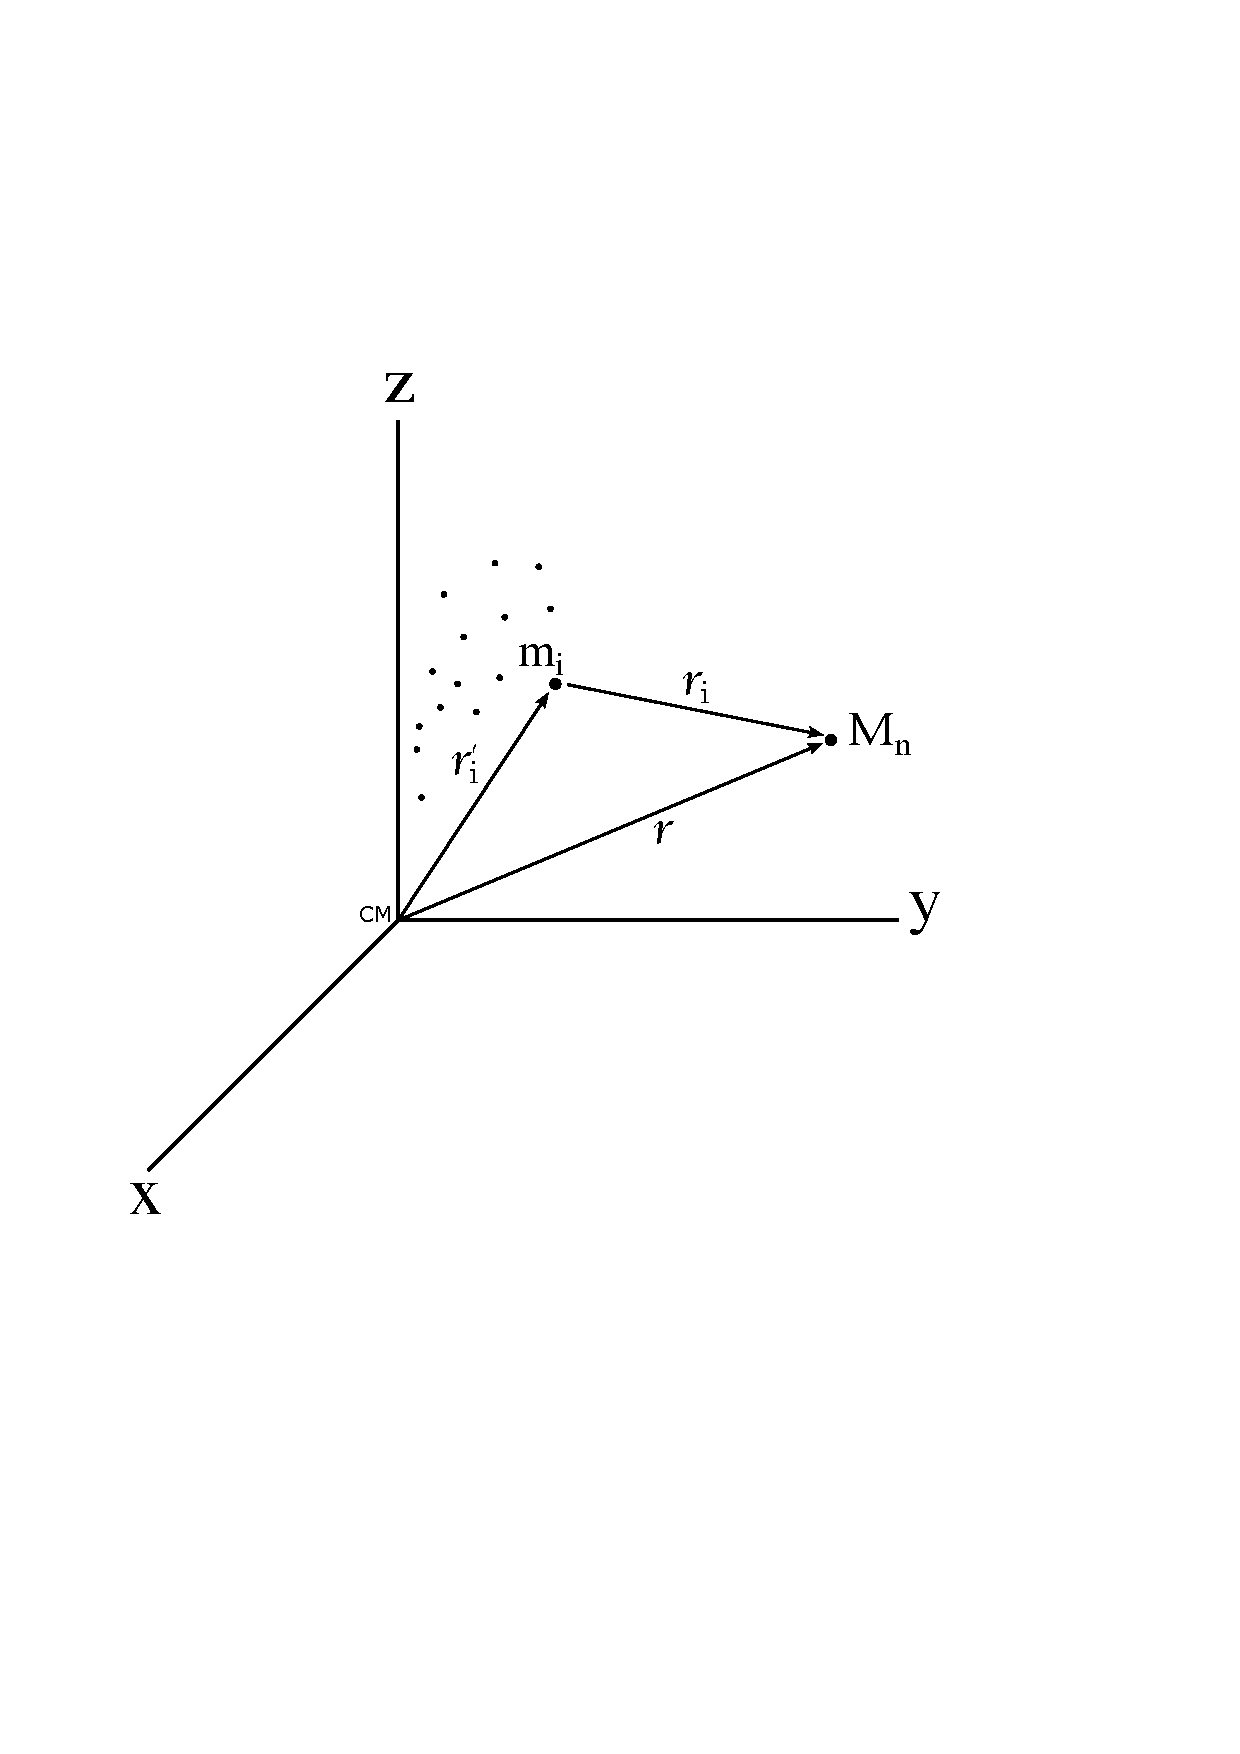
\includegraphics[width=7cm]{../Tesis/Capitulo3/Figures/NewtonianCM.pdf}
%\caption{Mass distribution}
%\label{fig: massdistribution}
%\end{figure}
%
%The solution is given in terms of the Legendre polynomials $P_n(x)$,
%
%\begin{align*}
%	V = -\frac{GM_n}{r} \sum_{n=0} m_i\left(\frac{r_i'}{r}\right)^n P_n(\cos\psi)
%\end{align*}
%
%For a spherical body the only term, due to spherical symmetry, non zero is for $n = 0$. If one choose the center of mass of de body as the origin of coordinates, the term $n = 1$ vanishes.\\
%
%The term $n = 2$
%\begin{align*}
%	V &= -\frac{GM_n}{r}  m_i\left(\frac{r_i'}{r}\right)^2 P_2(\cos\psi)\\
%	&=- \frac{GM_n}{2r^3}  m_i r_i^{'2} (3\cos^2\psi_i-1)\\
%	&= -\frac{GM_n}{2r^3}  m_i r_i^{'2} (2-3\sin^2\psi_i)
%\end{align*}
%where 
%\begin{align*}
%m_i r_i^{'2}\sin^2\psi_i = m_i r_i^{'2}(1-\cos^2\psi_i )= m_i \left(r_i^{'2} - \frac{(\mathbf{r_i'}\cdot \mathbf{r})^2}{r^2}\right) 
%\end{align*}
%
%The moment of inertia about the axis of rotation is $\mathcal{I}= \mathcal{I}_x\alpha^2+ \mathcal{I}_y\beta^2+ \mathcal{I}_z\gamma^2$, where $\alpha, \beta, \gamma$ are the direction cosines of the axis. This can be written as: 
%\begin{align}
%\label{eq: inertiamomentdiscrete}
%\mathcal{I}= m_i \left(r_i^{'2} - (\mathbf{r_i'}\cdot \mathbf{n})^2\right) 
%\end{align}
%by the other hand, the term
%\begin{align*}
%m_i r_i^{2} = m_i x_i^2+m_i y_i^2+m_i z_i^2
%\end{align*}
%and
%\begin{subequations}
%\begin{align*}
%\begin{gathered}
%\mathcal{I}_x = m_i (y_i^2 + z_i^2)\\
%\mathcal{I}_y = m_i (x_i^2 + z_i^2)\\
%\mathcal{I}_z = m_i (y_i^2 + x_i^2)\\
%\mathcal{I} = 2m_i(x_i^2+y_i^2+z_i^2) = 2m_ir_i^2
%\end{gathered}
%\end{align*}
%\end{subequations}
%The potential for $n = 2$
%\begin{align*}
%	V &= -\frac{GM_n}{2r^3} (\mathcal{I}_x + \mathcal{I}_y + \mathcal{I}_z -3\mathcal{I})
%\end{align*}
%If the symmetry axis is along the $z$ axis, then $\mathcal{I}_x = \mathcal{I}_y$. \cite{Goldstain}
%\begin{align*}
%	V &= -\frac{GM_n}{2r^3} (2\mathcal{I}_x  + \mathcal{I}_z -3(\mathcal{I}_x(\alpha^2 + \beta^2) + I_z\gamma^2)\\
%	&= -\frac{GM_n}{2r^3} (2\mathcal{I}_x  + \mathcal{I}_z -3(\mathcal{I}_x(1-\gamma^2) + \mathcal{I}_z\gamma^2)\\
%	&= -\frac{GM_n}{2r^3} (2\mathcal{I}_x  + \mathcal{I}_z -3(\mathcal{I}_z - \mathcal{I}_x)\gamma^2 -3\mathcal{I}_x)\\
%	&= -\frac{GM_n}{2r^3} (\mathcal{I}_z - \mathcal{I}_x)(1-3\gamma^2)
%\end{align*}
%The potential per unit mass until $ n = 2$
%\begin{align}
%\notag
%	U &=  -\frac{mc^2}{r}+\frac{G}{2r^3} (\mathcal{I}_x - \mathcal{I}_z)(1-3\cos^2\theta)\\
%\label{eq: weyllevicivitapotential}
%	U &=  -\frac{mc^2}{r}+\frac{Q}{2r^3} (1-3\cos^2\theta)
%\end{align}
%Compare with (\ref{eq: potentialWLC}), the quadrupole moment is \cite{Brumberg}:
%\begin{align}
%\label{eq: Q = G(A-C)}
%	Q = G(\mathcal{I}_x - \mathcal{I}_z) = \frac{2q}{15}m^3 c^2 
%\end{align}



%where $x^k$ is the component of the vector that gives the distance between the center of mass of the gravitational body and a point in the source. \\
%where $x^k$ is the component of the vector that gives the distance between the center of mass of the gravitational body and a test particle. ?????? SII???? 

It is possible to write the metric for the slowly rotating spheroid with the general post newtonian metric given in (\ref{eq:finalmetricpn}) as
%\begin{subequations}
%\begin{align}
% 			g_{00} &= -1-\frac{2}{c^{\hspace{0.05cm}2}}\phi -\frac{2}{c^2}\left(\frac{\phi^2}{c^2}+\psi \right) + \mathcal{O}(\epsilon^6) \\
% 			g_{0j} &= \frac{4}{c^{\hspace{0.05cm}3}}\zeta^j + \mathcal{O}(\epsilon^5) \\
%  			g_{jk} &= \left(1-\frac{2}{c^{\hspace{0.05cm}2}}\phi \right) \delta _{jk} + \mathcal{O}(\epsilon^4) 
%	\end{align}
%\end{subequations}

\begin{subequations}
\label{eq: hmunuslowlyrotation}
\begin{align}
 			h_{00} &= {}^{(2)}h_{00} + {}^{(4)}h_{00} + \mathcal{O}(\epsilon^6) 
			=-\frac{2}{c^{\hspace{0.05cm}2}}\phi -\frac{2}{c^2}\left(\frac{\phi^2}{c^2}+\psi \right) + \mathcal{O}(\epsilon^6) \\
 			h_{0j} &= {}^{(3)}h_{0j}  + \mathcal{O}(\epsilon^5) 
			= \frac{4}{c^{\hspace{0.05cm}3}}\zeta^j +  \partial_0 \partial_k \chi + \mathcal{O}(\epsilon^5) \\
  			h_{jk} &= {}^{(2)}h_{jk} + \mathcal{O}(\epsilon^4) 
			= \left(1-\frac{2}{c^{\hspace{0.05cm}2}}\phi \right) \delta _{jk} + \mathcal{O}(\epsilon^4) 
	\end{align}
\end{subequations}

The gravitational field of a slowly rotating spheroid can be characterized by the potential described above (\ref{eq: potentialphicomplete}), the vector potential $\zeta^j$ described in Chapter \ref{ch: firstchapter} in (\ref{eq: vector potential}) and the $\psi$ potential given in (\ref{eq: psipotential4hoo}).\\

	
%The newtonian potential is the one given in (\ref{eq: potentialphicomplete}).


\subsection{Vector potential}
 The vector potential is defined as
 \begin{align}
	\zeta^j &= -\frac{G}{c^{\hspace{0.05cm}2}}\int \frac{T^{\hspace{0.05cm}0j}(\mathbf{x'})}{|\mathbf{x}-\mathbf{x'}|}d^{\hspace{0.05cm}3}x' ,
\end{align}

where $\mathbf{x}$ is the vector between the center of mass of the gravitational body and the test particle, and the domain of integration extends over the volumen occupied by the source. %$\mathbf{x'}$ the distance to the center of mass to a point inside the gravitational body.\\

Expand the term $|\mathbf{x}-\mathbf{x'}|^{-1}$ in a Taylor series
\begin{align}
\frac{1}{|\mathbf{x}-\mathbf{x'}|} = \frac{1}{r} - x^{'l}\partial_l \left(\frac{1}{r}\right) + \frac{1}{2}x^{'l}x^{'m}\partial_l \partial_m \left(\frac{1}{r}\right) + ...
\label{eq: 1/xx'taylorexpansion}
\end{align}

%If $\mathbf{x}$ is the vector between the center of mass of the gravitational body and the test particle and $\mathbf{x'}$ the distance to the center of mass to a point inside the gravitational body, then $r' << r$, where $|\mathbf{x}| = r$ Expand the term $|\mathbf{x}-\mathbf{x'}|^{-1}$ in powers of $r'/r << 1$.
%
% \begin{align}
%	 \frac{1}{|\mathbf{x}-\mathbf{x'}|} &= \frac{1}{(r^2+r^{'2} - 2\mathbf{x} \cdot \mathbf{x'})^{1/2}} = \frac{1}{r}\left[1+\left( \frac{r'}{r}\right)^2 - 2\frac{\mathbf{x} \cdot \mathbf{x'}}{r^2}\right]^{-1/2}\\
%	 &=\frac{1}{r}\left[1-\frac{1}{2}\left( \frac{r'}{r}\right)^2 +\frac{\mathbf{r} \cdot \mathbf{r'}}{r^2}+...\right]
%\end{align}

the energy momentum component $T^{\hspace{0.05cm}0j}$ in (\ref{eq: Toiused}), then the vector potential in terms of the velocity of the source is

 \begin{align}
 \begin{split}
	\zeta^j = -G\int \frac{\rho(\mathbf{x'}) v^{'j}}{|\mathbf{x}-\mathbf{x'}|}d^{\hspace{0.05cm}3}x'  &= -\frac{G}{r} \int \rho(\mathbf{x'}) v^{'j}d^{\hspace{0.05cm}3}x' - \frac{Gx^{m}}{r^3} \int \rho(\mathbf{x'}) x^{'m} v^{'j}d^{\hspace{0.05cm}3}x',
\end{split}
\end{align}
where the velocity of the rotating spheroid is
\begin{align}
\label{eq: velocityslowly}
	v^{\,j} = \epsilon_{ijk} \omega^{\,j} x^{\,k}
\end{align}

% \begin{align}
% \begin{split}
%	\zeta^j = -G\int \frac{\rho(\mathbf{x'}) v^{'j}}{|\mathbf{x}-\mathbf{x'}|}d^{\hspace{0.05cm}3}x'  &= -\frac{G}{r} \int \rho(\mathbf{x'}) v^{'j}d^{\hspace{0.05cm}3}x' + \frac{G}{2r^3} \int \rho(\mathbf{x'}) x^{'2} v^{'j}d^{\hspace{0.05cm}3}x'\\
%	&- \frac{G x^{m}}{r^3} \int \rho(\mathbf{x'}) x^{'m} v^{'j}d^{\hspace{0.05cm}3}x'
%\end{split}
%\end{align}

The first term is null, due to the definition of center of mass,
\begin{align*}
	\int \rho(\mathbf{x'}) v^{'j}d^{\hspace{0.05cm}3}x' = \frac{d}{dt}  \int \rho(\mathbf{x'}) x^{'j}d^{\hspace{0.05cm}3}x' = 0.
\end{align*}
For the second term, 
\begin{align*}
	-\frac{Gx^{m}}{r^3} \int \rho(\mathbf{x'}) x^{'m} v^{'j}d^{\hspace{0.05cm}3}x' = -\epsilon_{jik}  \frac{Gx^{m}\omega^i}{r^3} \int \rho(\mathbf{x'}) x^{'m} x^{'k}d^{\hspace{0.05cm}3}x'
\end{align*}

Since the term inside the integral is the non-traceless inertia moment given in (\ref{eq: nontraclessinertiamoment}), the vector potential is 
 \begin{align}
	\zeta^j 
	& = -\frac{G}{r^3}\epsilon_{jik} \omega^i q^{\,km} x^{m}.
\end{align}

For a axially symmetric body and a rotation around the $z$-axis, the angular velocity is just
\begin{align}
\omega = \omega^3.
\end{align} 


The components of the vector potential, in terms of (\ref{eq: inertiamomentobrumberchipotential}), are
\begin{subequations}
\label{eq: componentsvectorpotential}
%\begin{empheq}[left=\empheqlbrace, right=\empheqrbrace]{align}
 \begin{align}
	 \zeta^1
	& = \frac{G C\omega  }{2r^3}y \\
	\zeta^2
	& = -\frac{G C\omega  }{2r^3}x \\
	\zeta^3 & = 0.
%\end{empheq}
\end{align}
\end{subequations}


%Consider a axially symmetric body and a rotation around the z-axis, the moments of inertia in the x and y axis are equal $I^{11} =I^{22} $. The vector potential can be written as
% \begin{align}
%	\zeta^j 
%	& = \frac{G}{r^3}\epsilon_{jik} \omega^i I^{km} x^{m} 
%\end{align}

\subsection{Potential $\psi$}

The potential $\psi$ is given in (\ref{eq: psipotential4hoo}),
\begin{align}
&\psi = -\frac{G}{c^{\hspace{0.05cm}2}}\int \frac{1}{|\mathbf{x}-\mathbf{x'}|}{}[^{(2)}T{}^{\hspace{0.07cm}00}(t,\mathbf{x'})+^{(2)}T{}^{\hspace{0.07cm}jj}(t,\mathbf{x'})]d^{\hspace{0.07cm}3}x' .
\end{align}

The energy-momentum components $^{(2)}T{}^{\hspace{0.07cm}00}$ and $^{(2)}T{}^{\hspace{0.07cm}jj}$ are given in (\ref{eq: Toiused}) by the expansion of the Lorentz factor $\gamma$,
\begin{align}
	\gamma(v) = U^0 = \frac{dt}{d\tau},
\end{align}
where $U^0 $ is the temporal component of the four-velocity and $\frac{dt}{d\tau}$ can be written as given in (\ref{eq:dtaudt}). Dropping $\mathcal{O}(\epsilon^4)$ and higher orders,
\begin{align}
	\gamma(v) = 1+\frac{v^2}{2c^2}+\frac{1}{2}{}^{(2)}h_{00}+\mathcal{O}(\epsilon^4).
\end{align}
Then, 
\begin{align}
 ^{(2)}T{}^{\hspace{0.07cm}00} &= \rho c^2 \left(\frac{v^2}{c^2} - \frac{2\phi}{c^2}\right),
\end{align}

where the term $v^2$ is neglected,
\begin{align*}
	v^2 = (\epsilon_{ijk} \omega^j x^k)\cdot (\epsilon_{ijk} \omega^j x^k) \sim \omega^2.
\end{align*}
The ${}^{(2)}T{}^{\hspace{0.07cm}jj}$ term is neglected,
\begin{align}
 c^{-2}{}^{(2)}T{}^{\hspace{0.07cm}jj} &= \rho v^j v^j 
\end{align}
\begin{align*}
	v^j v^j = (\epsilon_{jik} \omega^i x^k)\cdot (\epsilon_{jik} \omega^i x^k) \sim \omega^2.
\end{align*}


The $\psi$ potential up to first order of approximation in $\omega$ is
\begin{align}
\notag
\psi &= -G\int \frac{1}{|\mathbf{x}-\mathbf{x'}|} \rho(\mathbf{x'})\left(- \frac{2\phi}{c^2}\right)d^{\hspace{0.07cm}3}x'\\
&= \frac{2G}{c^{\hspace{0.05cm}2}}\int \frac{1}{|\mathbf{x}-\mathbf{x'}|} \rho(\mathbf{x'})\phi(\mathbf{x'}) d^{\hspace{0.07cm}3}x'.
\end{align}

Expand the term $|\mathbf{x}-\mathbf{x'}|^{-1}$ as in (\ref{eq: 1/xx'taylorexpansion})
\begin{align*}
\psi &= \frac{2G}{c^{\hspace{0.05cm}2}}\left[ \frac{1}{r} \int \rho(\mathbf{x'})\phi(\mathbf{x'}) d^{\hspace{0.07cm}3}x'  - \partial_m\left(\frac{1}{r}\right) \int \rho(\mathbf{x'})\phi(\mathbf{x'}) x^{'m}d^{\hspace{0.07cm}3}x'  \right] + ...\\
&= \frac{2G}{c^{\hspace{0.05cm}2}}\left[ \frac{1}{r} \int \rho(\mathbf{x'})\phi(\mathbf{x'}) d^{\hspace{0.07cm}3}x'  + \frac{x^m}{r^3} \int \rho(\mathbf{x'})\phi(\mathbf{x'}) x^{'m}d^{\hspace{0.07cm}3}x'  \right] + ... \hspace{0.3cm} .
\end{align*}

Expand the potential $\phi(\mathbf{x'})$ 
\begin{align}
\phi(\mathbf{x'}) = \phi(\mathbf{x}) + (x^{'j} - x^j)\partial _j \phi (\mathbf{x}) + ...
\end{align}
to obtain

\begin{align*}
\psi &= \frac{2G}{c^{\hspace{0.05cm}2}}\left[ \frac{1}{r} \phi(\mathbf{x}) \int    \rho(\mathbf{x'}) d^{\hspace{0.07cm}3}x' +  \frac{1}{r}  \partial_k \phi(\mathbf{x}) \int  \rho(\mathbf{x'}) (x^{'k} - x^k) d^{\hspace{0.07cm}3}x' \right. \\
& \left.+ \frac{x^m}{r^3}\phi(\mathbf{x}) \int \rho(\mathbf{x'}) x^{'m}d^{\hspace{0.07cm}3}x' +\frac{x^m}{r^3} \partial_k  \phi(\mathbf{x}) \int \rho(\mathbf{x'}) (x^{'k} - x^k)  x^{'m}d^{\hspace{0.07cm}3}x' \right] + ... \hspace{0.3cm} .
\end{align*}

As usual, the terms $\int \rho(\mathbf{x}) x d^{\hspace{0.07cm}3} x = 0$ and $\int \rho(\mathbf{x}) d^{\hspace{0.07cm}3} x = M$,

\begin{align}
\notag
\psi &= \frac{2G}{c^{\hspace{0.05cm}2}}\left[ \frac{M}{r}  \phi(\mathbf{x}) -  \frac{M x^k}{r}  \partial_k \phi(\mathbf{x})  +\frac{x^m}{r^3} \partial_k  \phi(\mathbf{x}) \underbrace{\int \rho(\mathbf{x'}) x^{'k}   x^{'m}d^{\hspace{0.07cm}3}x' } _{q^{km}}\right]\\
\label{eq: psipotentialexpresion}
&= \frac{2m}{r}\left[  \phi(\mathbf{x}) -  x^k  \partial_k \phi(\mathbf{x})  +\frac{x^m}{M r^2} \partial_k  \phi(\mathbf{x}) q^{km}\right] .
\end{align}

The second term is
\begin{align}
\notag
x^k  \partial_k \phi(\mathbf{x})  &= x^k\left[ \frac{GM}{r^3} x^ k - \frac{3Q}{2r^5} x^k \left(1-\frac{3z^2}{r^2}\right) + \frac{Q}{2r^3}\left(-\frac{6z}{r^2} \delta^{kz}+ \frac{6z^2}{r^4}x^k\right)\right]\\
\label{eq: psipotentialsecondterm}
&= \frac{GM}{r} - \frac{3Q}{2r^3}\left(1-\frac{3z^2}{r^2}\right)
\end{align}

and the third term is

\begin{align}
\notag
\frac{x^m}{M r^2} \partial_k  \phi(\mathbf{x}) q^{km} &= \frac{x^m}{M r^2} q^{km} \left[ \frac{GM}{r^3} x^k + Q(r, M, G)\right]\\
\notag
&= \frac{q^{km} x^m}{ r^2}  \frac{G}{r^3} x^k + (Q^{\,2})\\
\notag
&= \frac{G}{r^5} \left( x^2 q^{11}  + y^2 q^{22}+ z^2 q^{33}\right) = \frac{G}{r^5} \left[\frac{C}{2}(x^2  + y^2 - z^2) + A z^2 \right]\\
\notag
&= \frac{G}{r^5} \left[\frac{C}{2}(r^2  - 2z^2) + A z^2 \right] \\%= \frac{GC}{2r^3}   + \frac{z^2}{r^5} \underbrace{G(A-C)}_{Q (\ref{eq: Q = G(A-C)})} \\
\label{eq: psipotentialthirdterm}
&= \frac{GC}{2r^3}   + \frac{Qz^2}{r^5},
\end{align}
where $ Q(r, M, G)$ refers to the term of the derivative $\partial_k  \phi(\mathbf{x})$ that has dependence on $Q$, and $Q^{\,2}$ to the term involving multiplication of the inertia moments.\\

Replace (\ref{eq: psipotentialsecondterm}), (\ref{eq: psipotentialthirdterm}) and the Newtonian potential in (\ref{eq: psipotentialexpresion}),
\begin{align}
\notag
\psi &= \frac{2m}{r}\left[ -\frac{GM}{r} + \frac{Q}{2r^3}\left(1-\frac{3z^2}{r^2}\right) - \frac{GM}{r}- \frac{3Q}{2r^3}\left(1-\frac{3z^2}{r^2}\right) + \frac{GC}{2r^3}   + \frac{Qz^2}{r^5} \right]\\
&= -\frac{4GMm}{r^2} + \frac{2Qm}{r^4}\left(2-\frac{5z^2}{r^2}\right) +\frac{GmC}{r^4}.
\end{align}

\subsection{Parametrized Metric}
With all the necessary elements, the metric given in (\ref{eq: hmunuslowlyrotation}) can be written, in components as
\begin{subequations}
\label{eq: metricnoparametrized} 
\begin{align}
&{}^{(2)}h_{00} = \frac{2m}{r} \frac{Q}{c^2r^3}\left(1-\frac{3z^2}{r^2}\right) \\
\notag
&{}^{(4)}h_{00} = \frac{6m^2}{r^2} - \frac{2Qm}{c^2 r^4}\left(3-\frac{7z^2}{r^2}\right) -\frac{2GmC}{c^2 r^4}\\
&\hspace{1cm} =\frac{6m^2}{r^2} - \frac{6Qm}{c^2 r^4}\left(1-\frac{3z^2}{r^2}\right)  - \frac{4Qm}{c^2 r^4}\frac{z^2}{r^2}-\frac{2GmC}{c^2 r^4}\\
&{}^{(3)}h_{01} = \frac{2GC\omega}{c^3 r^3}y\\
&{}^{(3)}h_{02} = -\frac{2GC\omega}{c^3 r^3}x\\
&{}^{(3)}h_{03} = 0\\
&{}^{(2)}h_{ij} = \frac{2m}{r}\delta_{ij} - \frac{Q}{c^2 r^3}\left(1-\frac{3z^2}{r^2}\right) \delta_{ij}.
\end{align}
\end{subequations}

It is convenient to parameterize this metric, just as did in Chapter \ref{ch:chapter2},
\begin{subequations}
\label{eq: metricparametrized}
\begin{align}
&{}^{(2)}h_{00} = \frac{2m}{r} \frac{Q}{c^2r^3}\left(1-\frac{3z^2}{r^2}\right)\\
\begin{split}
&{}^{(4)}h_{00} = 2[3 + (\alpha - 4)\beta ]\frac{m^2}{r^2} - [6+(3\alpha - 8)\beta] \frac{Qm}{c^2 r^4}\left(1-\frac{3z^2}{r^2}\right)  \\ 
&\hspace{1cm}- 4(1-\beta )\frac{Qm}{c^2 r^4}\frac{z^2}{r^2}-2(1-\beta )\frac{GmC}{c^2 r^4}
\end{split}
\end{align}
\begin{align}
&{}^{(3)}h_{01} = \frac{2GC\omega}{c^3 r^3}y\\
&{}^{(3)}h_{02} = -\frac{2GC\omega}{c^3 r^3}x\\
&{}^{(3)}h_{03} = 0\\
&{}^{(2)}h_{ij} = 2(1-\alpha\beta)\frac{2m}{r}\delta_{ij} + 2\alpha\beta \frac{m}{r^3}x^i x^j- \frac{Q}{c^2 r^3}\left(1-\frac{3z^2}{r^2}\right) \delta_{ij}.
\end{align}
\end{subequations}

Note here that with $\beta = 0$ the metric in (\ref{eq: metricparametrized}) recovers (\ref{eq: metricnoparametrized}), and with $\beta = 1$ the metric reduces to that found in \cite{Brumberg}.


\section{Construction of the Perturbing Force}
\subsection{Lagrangian}

Consider the Lagrangian described in the equation (\ref{eq:firstlagrangian}) and replace the metric given in (\ref{eq: metricparametrized}),

%\begin{align*}
%L &= \frac{1}{2}  \dot{\mathbf{x}}^2 + \frac{1}{2}c^{2(2)}h_{00} + \frac{1}{8}  \frac{(\dot{\mathbf{x}}^{2})^2}{c^2}  + \frac{1}{2} c^{2(4)}h_{00} +  c^{(3)}h_{0j} \dot{x}^j \\
%&+ \frac{1}{2}{}^{(2)}h_{ij}\dot{x}^{i} \dot{x}^{j} + \frac{1}{8}c^{2}\left(^{(2)}h_{00} \right)^{2} + \frac{1}{4}{}^{(2)}h_{00} \dot{\mathbf{x}}^2 + \mathcal{O}(\epsilon^3)
%\end{align*}

\begin{align}
%\begin{split}
\notag
L &= \frac{1}{2}  \dot{\mathbf{x}}^2 + \frac{1}{2}c^{2}\left[\frac{2m}{r} -\frac{Q}{r^3 c^2}\left(1-\frac{3z^2}{r^2}\right)\right] + \textcolor{red}{\frac{1}{8}  \frac{(\dot{\mathbf{x}}^{2})^2}{c^2}}+
 \frac{1}{2} c^{2} \left[\textcolor{red}{2[3 + (\alpha - 4)\beta ]\frac{m^2}{r^2} }  \right. \\ \notag \\ \notag
 &\left. \textcolor{morado}{- [6+(3\alpha - 8)\beta] \frac{Qm}{c^2 r^4}\left(1-\frac{3z^2}{r^2}\right)
 - 4(1-\beta )\frac{Qm}{c^2 r^4}\frac{z^2}{r^2}}\textcolor{morado}{-2(1-\beta )\frac{GmC}{c^2 r^4}}\right] \\
\notag \\ \notag
&+  \textcolor{cadmiumorange}{c \left[-\frac{2GC\omega}{c^3r^3}(x\dot{y} - y\dot{x})\right] } 
+ \frac{1}{2}\left[\textcolor{red} {2(1-\alpha\beta)\frac{m}{r} \delta _{jk}  + 2\alpha\beta \frac{m}{r^3}x^jx^k} \textcolor{morado}{-\frac{Q}{r^3 c^2}\left(1-\frac{3z^2}{r^2}\right) \delta _{jk} }\right]\dot{x}^{j} \dot{x}^{k} \\ \notag \\
&+ \frac{1}{8}c^{2}\left[\textcolor{red}{\frac{4m^2}{r^2}} \textcolor{morado}{-\frac{4Qm}{c^2r^4}\left(1-\frac{3z^2}{r^2}\right)}\right] + \frac{1}{4}\left[\textcolor{red}{\frac{2m}{r}} \textcolor{morado}{-\frac{Q}{r^3 c^2}\left(1-\frac{3z^2}{r^2}\right)}\right] \dot{\mathbf{x}}^2 + \mathcal{O}(\epsilon^3, Q^2).
%\end{split} 
\end{align}

Grouping terms,
\begin{subequations}
\begin{align}
\notag
L_2 =& \textcolor{red}{\frac{1}{8}  \frac{(\dot{\mathbf{x}}^{2})^2}{c^2}  + [3 + (\alpha - 4)\beta ]c^2\frac{m^2}{r^2}  
+(1-\alpha\beta)\frac{m}{r} \delta _{jk} \dot{x}^{j} \dot{x}^{k} + \alpha\beta \frac{m}{r^3}x^jx^k  \dot{x}^{j} \dot{x}^{k} 
+\frac{1}{2}\frac{m^2c^2}{r^2} + \frac{m}{2r}\dot{\mathbf{x}}^2}\\ \notag \\
\notag
=&\frac{1}{8}  \frac{(\dot{\mathbf{x}}^{2})^2}{c^2} + \dot{\mathbf{x}}^2\left[\frac{m}{2r} + (1-\alpha \beta)\frac{m}{r} \right] + \frac{c^2m^2}{r^2}\left[(3+ (\alpha-4)\beta) + \frac{1}{2}\right] + \frac{\alpha \beta m}{r^3} (\mathbf{x}\cdot\dot{\mathbf{x}})^2 \\ \notag \\
=&\frac{1}{8}  \frac{(\dot{\mathbf{x}}^{2})^2}{c^2}  + \frac{m}{r}  \left[ \left(\frac{3}{2} - \alpha \beta \right)\dot{\mathbf{x}}^2 + c^2 \frac{m}{r}\left(\frac{7}{2} + (\alpha-4)\beta \right) + \alpha \beta \frac{(\mathbf{x}\cdot\dot{\mathbf{x}})^2}{r^2}\right]\\ \notag \\
L_3 =& \textcolor{cadmiumorange}{c \left[-\frac{2GC\omega}{c^3r^3}(x\dot{y} - y\dot{x})\right] }\\
\notag \\ \notag
L_4 =& \textcolor{morado}{- [6+(3\alpha - 8)\beta] \frac{Qm}{2 r^4}\left(1-\frac{3z^2}{r^2}\right)
 - 2(1-\beta )\frac{Qm}{r^4}\frac{z^2}{r^2} - \frac{Q}{2r^3c^2}\left(1-\frac{3z^2}{r^2}\right)\dot{\mathbf{x}}^2} \\
\notag
&\textcolor{morado}{-\frac{Qm}{2r^4} \left(1-\frac{3z^2}{r^2}\right) - \frac{Q}{4r^3c^2}\left(1-\frac{3z^2}{r^2}\right)\dot{\mathbf{x}}^2 - (1-\beta)\frac{GmC}{r^4}}\\
\notag \\ \notag
=&\frac{Q}{2c^2r^3}\left(1-\frac{3z^2}{r^2}\right)\left[-\frac{3}{2}\dot{\mathbf{x}}^2 - [7+(3\alpha-8)\beta] \frac{mc^2}{r}\right] - 2(1-\beta )\frac{Qm}{r^4}\frac{z^2}{r^2} - (1-\beta)\frac{GmC}{r^4}
\end{align}
\end{subequations}

The Lagrangian is given by
\begin{align}
L = L_0 + L_1+L_2+L_3+L_4
\end{align}
where

\begin{subequations}
\label{eq: lagrangianslowlyrotation}
\begin{align}
 L_0 =& \frac{1}{2}  \dot{\mathbf{x}}^2 + \frac{GM}{r} \\
 L_1 =& -\frac{Q}{2r^3}\left(1-\frac{3z^2}{r^2}\right)\\
 L_2 =&\frac{1}{8}  \frac{(\dot{\mathbf{x}}^{2})^2}{c^2}  + \frac{m}{r}  \left[ \left(\frac{3}{2} - \alpha \beta \right)\dot{\mathbf{x}}^2 + c^2 \frac{m}{r}\left(\frac{7}{2} + (\alpha-4)\beta \right) + \alpha \beta \frac{(\mathbf{x}\cdot\dot{\mathbf{x}})^2}{r^2}\right]\\
 L_3 =& -\frac{2GC\omega}{c^2r^3}(x\dot{y} - y\dot{x}) \\
 L_4 =& \frac{Q}{2c^2r^3}\left(1-\frac{3z^2}{r^2}\right)\left[-\frac{3}{2}\dot{\mathbf{x}}^2 - [7+(3\alpha-8)\beta] \frac{mc^2}{r}\right] \\
 -& 2(1-\beta )\frac{Qm}{r^4}\frac{z^2}{r^2} - (1-\beta)\frac{GmC}{r^4}
 \end{align}
\end{subequations}

\section{Perturbing Force}

With the Lagrangian given above calculate the perturbing force, via the Euler Lagrange equations. The term $L_0$ is the Newtonian contribution, i.e.,it  is not part of the perturbation. Although the perturbing forces do not arise from a potential, those forces can be found by
\begin{align}
F = \frac{\partial L}{\partial \mathbf{x}} - \frac{d}{dt}\left(\frac{\partial L}{\partial \dot{\mathbf{x}} }\right).
\end{align}

For $L_1$, the Euler Lagrange equations give
\begin{align*}
	 \mathbf{F_1} = \frac{\partial}{\partial{\mathbf{x}}} \left[-\frac{Q}{2r^3}\left(1-\frac{3z^2}{r^2}\right)\right] - \frac{d}{dt}\left[\frac{\partial}{\partial{\dot{\mathbf{x}}}} \left(-\frac{Q}{2r^3}\left(1-\frac{3z^2}{r^2}\right)\right)\right]
\end{align*}

\begin{align*}
\notag
	\mathbf{F_1} &= -\frac{Q}{2}\left[-\frac{3}{r^5}\left(1-\frac{3z^2}{r^2}\right)\mathbf{x} + \frac{1}{r^3}\left(-\frac{6z}{r^2}\mathbf{\hat{e}_k} + \frac{6z^2}{r^4} \mathbf{x}\right)\right]\\
\notag
	&=\frac{3Q}{r^5}\left[\frac{1}{2}\left(1-\frac{3z^2}{r^2}\right)\mathbf{x} + z\mathbf{\hat{e}_k} - \frac{z^2}{r^2}\mathbf{x}\right]\\
%\label{eq: F_1}
	&=\frac{3Q}{r^5} \left[\frac{1}{2}\left(1-\frac{5z^2}{r^2}\right)\mathbf{x} + z\mathbf{\hat{e}_k}\right].
\end{align*}

For $L_2$, the Euler Lagrange equations give
\begin{align*}
	 \mathbf{F_2}
=& \frac{\partial}{\partial{\mathbf{x}}} \left\{  \frac{m}{r}  \left[ \left(\frac{3}{2} - \alpha \beta \right)\dot{\mathbf{x}}^2 + c^2 \frac{m}{r}\left(\frac{7}{2} + (\alpha-4)\beta \right) + \alpha \beta \frac{(\mathbf{x}\cdot\dot{\mathbf{x}})^2}{r^2}\right]\right\} \\
	&- \frac{d}{dt}\left\{\frac{\partial}{\partial{\dot{\mathbf{x}}}} \left(\frac{1}{8}  \frac{(\dot{\mathbf{x}}^{2})^2}{c^2}  + \frac{m}{r}  \left[ \left(\frac{3}{2} - \alpha \beta \right)\dot{\mathbf{x}}^2 +  \alpha \beta \frac{(\mathbf{x}\cdot\dot{\mathbf{x}})^2}{r^2}\right]\right)\right\}.  
\end{align*}

The derivative with respect to $\mathbf{x}$ is
\begin{align}
\notag
 \frac{\partial}{\partial{\mathbf{x}}}& \left\{  \frac{m}{r}  \left[ \left(\frac{3}{2} - \alpha \beta \right)\dot{\mathbf{x}}^2 + c^2 \frac{m}{r}\left(\frac{7}{2} + (\alpha-4)\beta \right) + \alpha \beta \frac{(\mathbf{x}\cdot\dot{\mathbf{x}})^2}{r^2}\right]\right\} \\
 \notag
& =  -\frac{m}{r^3}\left(\frac{3}{2}-\alpha \beta \right)\dot{\mathbf{x}}^{2} \mathbf{x} - \frac{2GMm}{r^4}\left(\frac{7}{2}+(\alpha-4)\beta \right)\mathbf{x} \\ 
 \label{eq: xderivativeF2}
 &=- \frac{3m\alpha \beta}{r^5} (\mathbf{x} \cdot \dot{\mathbf{x}})^2 \mathbf{x} + \frac{2m\alpha\beta}{r^3}(\mathbf{x} \cdot \dot{\mathbf{x}}) \mathbf{x}.
\end{align}

For the derivative with respect to $t$, let see the first term,
\begin{align*}
&\frac{d}{dt}\left\{\frac{\partial}{\partial{\dot{\mathbf{x}}}} \left(\frac{1}{8}  \frac{(\dot{\mathbf{x}}^{2})^2}{c^2}\right)\right\} = \frac{d}{dt}\left\{\frac{\partial}{\partial{\dot{\mathbf{x}}}} \left(\frac{1}{8}  \frac{(\dot{\mathbf{x}}\cdot \dot{\mathbf{x}})^2}{c^2}\right)\right\} =  \frac{d}{dt}\left\{\frac{2}{8}  \frac{(\dot{\mathbf{x}}\cdot \dot{\mathbf{x}}) (\dot{\mathbf{x}}+\dot{\mathbf{x}})}{c^2}\right\}\\
&\frac{d}{dt}\left\{\frac{1}{2}  \frac{(\dot{\mathbf{x}}\cdot \dot{\mathbf{x}}) \dot{\mathbf{x}}}{c^2}\right\} = \frac{1}{2c^2}\left\{2(\ddot{\mathbf{x}} \cdot \dot{\mathbf{x}})\dot{\mathbf{x}} + (\dot{\mathbf{x}}\cdot \dot{\mathbf{x}})\ddot{\mathbf{x}}\right\}.
\end{align*}

The other terms in the temporal derivative,
\begin{align}
\notag
 \frac{d}{dt} &\left\{\frac{m}{r}  \left[ \left(\frac{3}{2} - \alpha \beta \right)\dot{\mathbf{x}}^2 +  \alpha \beta \frac{(\mathbf{x}\cdot\dot{\mathbf{x}})^2}{r^2}\right]\right\} \\ \notag
 &=  \underbrace{\frac{1}{2c^2}\left\{2(\ddot{\mathbf{x}} \cdot \dot{\mathbf{x}})\dot{\mathbf{x}} + (\dot{\mathbf{x}}\cdot \dot{\mathbf{x}})\ddot{\mathbf{x}}\right\}}_{\text{1.} \mathbf{F_4}} - \frac{2m}{r^3}\left(\frac{3}{2}-\alpha \beta \right) (\mathbf{x} \cdot \dot{\mathbf{x}}) \dot{\mathbf{x}} + \underbrace{\frac{2m}{r}\left(\frac{3}{2}-\alpha \beta \right)\ddot{\mathbf{x}}}_{\text{2.} \mathbf{F_4}}- \frac{6m\alpha \beta }{r^5}(\mathbf{x} \cdot \dot{\mathbf{x}})^2 \mathbf{x} \\
 \label{eq: temporalpartofF2}
& + \frac{2m\alpha \beta}{r^3}\left[(\dot{\mathbf{x}} \cdot \dot{\mathbf{x}}) \mathbf{x} + \underbrace{(\mathbf{x} \cdot \ddot{\mathbf{x}}) \mathbf{x}}_{\text{3.}  \mathbf{F_4}} + (\mathbf{x} \cdot \dot{\mathbf{x}}) \dot{\mathbf{x}} \right].
 \end{align}
 
 The second derivative $\ddot{\mathbf{x}}$ in the equations above, according to (\ref{eq:equationsofmotion}), can be written as 
 \begin{align*}
 \ddot{\mathbf{x}} = -\nabla \phi ,
 \end{align*}
where $\phi$ is given by (\ref{eq: potentialphicomplete})
 \begin{align}
 \label{eq: ddotxcontributionforforce}
 \ddot{\mathbf{x}} =  -\nabla \left[-\frac{mc^2}{r} + \frac{Q}{2r^3}\left(1-\frac{3z^2}{r^2}\right) \right] = -\frac{GM}{r^3}\mathbf{x}  - \nabla \left[\frac{Q}{2r^3}\left(1-\frac{3z^2}{r^2}\right) \right].
\end{align}
To preserve the order of this contribution (without $Q$), we only consider the first term of $\ddot{\mathbf{x}}$, then (\ref{eq: temporalpartofF2}) becomes
%\begin{subequations}
\begin{align}
\notag 
&\frac{1}{2c^2}\left\{-2\frac{GM}{r^3}(\mathbf{x} \cdot \dot{\mathbf{x}})\dot{\mathbf{x}} - \frac{GM}{r^3}(\dot{\mathbf{x}}\cdot \dot{\mathbf{x}})\mathbf{x}\right\} - \frac{2m}{r^3}\left(\frac{3}{2}-\alpha \beta \right) (\mathbf{x} \cdot \dot{\mathbf{x}}) \dot{\mathbf{x}} - \frac{2GMm}{r^4}\left(\frac{3}{2}-\cancel{\alpha \beta}\right)\mathbf{x} \\  \notag \\
 \notag 
 &\hspace{1cm}- \frac{6m\alpha\beta}{r^5}(\mathbf{x} \cdot \dot{\mathbf{x}})^2 \mathbf{x}  + \frac{2m\alpha\beta}{r^3}\left[(\dot{\mathbf{x}} \cdot \dot{\mathbf{x}}) \mathbf{x} -\cancel{\frac{GM}{r^3} (\mathbf{x} \cdot \mathbf{x}) \mathbf{x}} + (\mathbf{x} \cdot \dot{\mathbf{x}}) \dot{\mathbf{x}} \right] \\ \notag\\ 
% \end{align*}
 %\begin{align}
  \notag 
 &=  \frac{1}{2c^2}\left\{-2\frac{GM}{r^3}(\mathbf{x} \cdot \dot{\mathbf{x}})\dot{\mathbf{x}} - \frac{GM}{r^3}(\dot{\mathbf{x}}\cdot \dot{\mathbf{x}})\mathbf{x}\right\} \textcolor{forestgreen}{- \frac{2m}{r^3}\left(\frac{3}{2}-\alpha \beta \right) (\mathbf{x} \cdot \dot{\mathbf{x}}) \dot{\mathbf{x}} }- \frac{3GMm}{r^4}\mathbf{x} \\  \notag \\  \notag 
 & \hspace{1cm}- \frac{6m\alpha\beta}{r^5}(\mathbf{x} \cdot \dot{\mathbf{x}})^2 \mathbf{x}  + \frac{2m\alpha\beta}{r^3}\left[(\dot{\mathbf{x}} \cdot \dot{\mathbf{x}}) \mathbf{x}  +\textcolor{forestgreen}{ (\mathbf{x} \cdot \dot{\mathbf{x}}) \dot{\mathbf{x}} }\right]\\   \notag \\   \notag
 %\begin{split}
 &= -\frac{m}{r^3} (\mathbf{x} \cdot \dot{\mathbf{x}})\dot{\mathbf{x}} -\frac{m}{2r^3}  \dot{\mathbf{x}}^2 \mathbf{x} - \frac{3GMm}{r^4}\mathbf{x} + \frac{2m\alpha\beta}{r^3}\dot{\mathbf{x}}^2 \mathbf{x}  - \frac{6m\alpha\beta}{r^5}(\mathbf{x} \cdot \dot{\mathbf{x}})^2 \mathbf{x} \\  \notag \\
  \label{eq: timederivativeF2}
 &\hspace{1cm} \textcolor{forestgreen}{ - \frac{2m}{r^3}\left(\frac{3}{2}-2\alpha \beta \right) (\mathbf{x} \cdot \dot{\mathbf{x}}) \dot{\mathbf{x}} }.
% \end{split}
 \end{align}
 %\end{subequations}
 The second term in (\ref{eq: ddotxcontributionforforce}) (with $Q$) is going to be used for the $\mathbf{F}_4$ contribution.\\
 
Adding (\ref{eq: xderivativeF2}) and (\ref{eq: timederivativeF2})
 %\begin{subequations}
 \begin{align*}
 \notag
 \mathbf{F_2} =& \textcolor{red}{-\frac{m}{r^3}\left(\frac{3}{2}-\alpha \beta \right)\dot{\mathbf{x}}^{2} \mathbf{x}} \textcolor{cadmiumorange}{- \frac{2GMm}{r^4}\left(\frac{7}{2}+(\alpha-4)\beta \right)\mathbf{x}}  \textcolor{blue}{-\frac{3m\alpha\beta}{r^5} (\mathbf{x} \cdot \dot{\mathbf{x}})^2 \mathbf{x} }+ \textcolor{forestgreen}{\frac{2m\alpha\beta}{r^3}(\mathbf{x} \cdot \dot{\mathbf{x}}) \mathbf{x}}\\  \notag \\
  \notag
 & \textcolor{forestgreen}{+ \frac{m}{r^3}(\mathbf{x} \cdot \dot{\mathbf{x}})\dot{\mathbf{x}}} \textcolor{red}{+ \frac{m}{r^3} \dot{\mathbf{x}}^2 \mathbf{x}}  \textcolor{forestgreen}{- \frac{2m}{r^3}\left(\frac{3}{2}-2\alpha\beta\right) (\mathbf{x} \cdot \dot{\mathbf{x}}) \dot{\mathbf{x}}} \textcolor{cadmiumorange}{+\frac{3GMm}{r^4}\mathbf{x}} \\ \notag \\ \notag
 &\textcolor{blue}{+ \frac{6m\alpha \beta }{r^5}(\mathbf{x} \cdot \dot{\mathbf{x}})^2 \mathbf{x}}  \textcolor{red}{ - \frac{2m\alpha\beta}{r^3}(\dot{\mathbf{x}} \cdot \dot{\mathbf{x}}) \mathbf{x}} \\ \notag \\ \notag \\ \notag
%\end{align*}
 %\begin{align*}
 \mathbf{F_2} =& \textcolor{red}{-\frac{m}{r^3}\left(1+ \alpha \beta \right)\dot{\mathbf{x}}^{2} \mathbf{x}} + \textcolor{blue}{\frac{3m\alpha\beta}{r^5} (\mathbf{x} \cdot \dot{\mathbf{x}})^2 \mathbf{x} }\textcolor{forestgreen}{+ \frac{2m}{r^3}(2-\alpha \beta)(\mathbf{x} \cdot \dot{\mathbf{x}}) \mathbf{x}} + \textcolor{cadmiumorange}{ \frac{2GMm}{r^4}\left(-4+8\beta - 2\alpha\beta \right)\mathbf{x} }\\  \notag\\ \notag \\
% \label{eq: F_2}
 \mathbf{F_2} =& \frac{m}{r^3}\left\{\left[\frac{3\alpha\beta }{r^2} (\mathbf{x} \cdot \dot{\mathbf{x}})^2  + \frac{GM}{r}[-2\beta(\alpha-4) - 4] -  (1+\alpha\beta)\dot{\mathbf{x}}^{2} \right] \mathbf{x} +  (4-2\alpha\beta) (\mathbf{x} \cdot \dot{\mathbf{x}}) \dot{\mathbf{x}}\right\}.
\end{align*}

\newpage

For $L_3$, the Euler Lagrange equations give
 \begin{align*}
\mathbf{F_3} &= \frac{d}{d{\mathbf{x}}} \left\{-\frac{2GC\omega}{c^2r^3}(x\dot{y} - y\dot{x}) \right\} - \frac{d}{dt}\left\{\frac{d}{d{\dot{\mathbf{x}}}} \left(-\frac{2GC\omega}{c^2r^3}(x\dot{y} - y\dot{x}) \right)\right\}.
\end{align*}

Calculate the first term
 \begin{align*}
\mathbf{x} \times \dot{\mathbf{x}} = (y\dot{z}-z\dot{y}) \hat{\mathbf{i}} -  (x\dot{z}-z\dot{x}) \hat{\mathbf{j}} + (x\dot{y}-y\dot{x}) \mathbf{\hat{e}_k}
\end{align*}
and then, the equation can be written as

 \begin{align*}
\mathbf{F_{3}} &= \frac{\partial}{\partial{\mathbf{x}}} \left\{-\left[\frac{2GC\omega}{c^2r^3}(\mathbf{x} \times \dot{\mathbf{x}}) \cdot \mathbf{\hat{e}_k}\right]
\right\}- \frac{d}{dt}\left\{\frac{\partial}{\partial{\dot{\mathbf{x}}}} \left(-\left[\frac{2GC\omega}{c^2r^3}(\mathbf{x} \times \dot{\mathbf{x}}) \cdot \mathbf{\hat{e}_k}\right]\right)\right\}.
\end{align*}

To solve the derivatives, lets introduce the cross product in the matrix form,
\begin{align*}
	\mathbf{x} \times \dot{\mathbf{x}} = 
\begin{bmatrix}
0&-z&y\\
z&0&-x\\
-y&x&0
\end{bmatrix}
\cdot
\begin{bmatrix}
\dot{x}\\
\dot{y}\\
\dot{z}
\end{bmatrix}
=
\begin{bmatrix}
-z\dot{y} + y\dot{z} \\
z\dot{x}  - x\dot{z}\\
-y\dot{x} + x\dot{y}
\end{bmatrix}.
\end{align*}

This is notated as
\begin{align}
	\mathbf{x} \times \dot{\mathbf{x}} = [\mathbf{x}] \cdot \dot{\mathbf{x}}.
\end{align}
Hence,
 \begin{align*}
\mathbf{F_{3}} =& \frac{\partial}{\partial{\mathbf{x}}} \left\{-\left[\frac{2GC\omega}{c^2r^3}([\mathbf{x}] \cdot \dot{\mathbf{x}}) \cdot \mathbf{\hat{e}_k}\right]
\right\}- \frac{d}{dt}\left\{\frac{\partial}{\partial{\dot{\mathbf{x}}}} \left(-\left[\frac{2GC\omega}{c^2r^3}([\mathbf{x}] \cdot \dot{\mathbf{x}}) \cdot \mathbf{\hat{e}_k}\right]\right)\right\}\\ \\
=&\frac{2GC\omega}{c^2} \left\{\frac{3}{r^5} \mathbf{x}  (\mathbf{x} \times \dot{\mathbf{x}}) \cdot \mathbf{\hat{e}_k}-\frac{1}{r^3}[\dot{\mathbf{x}}] \cdot\mathbf{\hat{e}_k} \right\} + \frac{2GC\omega}{c^2} \frac{d}{dt}\left\{-\frac{1}{r^3}[\mathbf{x}]\cdot \mathbf{\hat{e}_k} \right\}\\ \\ 
=&\frac{2GC\omega}{c^2r^3} \left\{\frac{3}{r^2} \mathbf{x} (\mathbf{x} \times \dot{\mathbf{x}}) \cdot \mathbf{\hat{e}_k} -(\dot{\mathbf{x}} \times \mathbf{\hat{e}_k}) \right\} + \frac{2GC\omega}{c^2}\left\{\frac{3}{r^5} (\mathbf{x} \cdot  \dot{\mathbf{x}} )(\mathbf{x} \times\mathbf{\hat{e}_k}) - \frac{1}{r^3}(\dot{\mathbf{x}} \times  \mathbf{\hat{e}_k}) \right\}\\ \\
=&\frac{2GC\omega}{c^2r^3} \left\{\frac{3}{r^2}  \mathbf{x}  (\mathbf{x} \times \dot{\mathbf{x}}) \cdot \mathbf{\hat{e}_k} -2(\dot{\mathbf{x}} \times \mathbf{\hat{e}_k}) + \frac{3}{r^2} (\mathbf{x} \cdot \dot{\mathbf{x}} ) (\mathbf{x} \times \mathbf{\hat{e}_k})  \right\}\\ \\
=&\frac{2GC\omega}{c^2r^3} \left\{-2(\dot{\mathbf{x}} \times\mathbf{\hat{e}_k})+ \frac{3}{r^2}   x (x\dot{y} - y\dot{x}) \mathbf{\hat{e}_x}  + \frac{3}{r^2} (x\dot{x} + y\dot{y}+ z\dot{z})y  \mathbf{\hat{e}_x}  \right. \\
&\left. + \frac{3}{r^2}   y (x\dot{y} - y\dot{x}) \mathbf{\hat{e}_y}  - \frac{3}{r^2} (x\dot{x} + y\dot{y}+ z\dot{z})x  \mathbf{\hat{e}_y} + \frac{3z}{r^2}    (x\dot{y} - y\dot{x}) \mathbf{\hat{e}_z}
\right\}\\ \\
=&\frac{2GC\omega}{c^2r^3} \left\{-2(\dot{\mathbf{x}} \times\mathbf{\hat{e}_k}) + \frac{3}{r^2}(x^2+y^2)\dot{y}  \mathbf{\hat{e}_x}  + \frac{3}{r^2}yz\dot{z}  \mathbf{\hat{e}_x} - \frac{3}{r^2} (x^2+y^2) \dot{x} \mathbf{\hat{e}_y}- \frac{3}{r^2}xz\dot{z}\mathbf{\hat{e}_y} + \frac{3z}{r^2}    (x\dot{y} - y\dot{x}) \mathbf{\hat{e}_z}\right\}\\ \\
=&\frac{2GC\omega}{c^2r^3} \left\{-2(\dot{\mathbf{x}} \times\mathbf{\hat{e}_k}) + \frac{3}{r^2}(r^2-z^2) (\dot{y}  \mathbf{\hat{e}_x} - \dot{x}  \mathbf{\hat{e}_y} )+\frac{3z}{r^2} y\dot{z}  \mathbf{\hat{e}_x}  - \frac{3x}{r^2} x\dot{z}  \mathbf{\hat{e}_y}+ \frac{3z}{r^2}    (x\dot{y} - y\dot{x}) \mathbf{\hat{e}_z}\right\}\\ \\
=&\frac{2GC\omega}{c^2r^3} \left\{-2(\dot{\mathbf{x}} \times\mathbf{\hat{e}_k}) + 3 (\dot{y}  \mathbf{\hat{e}_x} - \dot{x}  \mathbf{\hat{e}_y} ) - \frac{3z}{r^2}(z\dot{y}  \mathbf{\hat{e}_x} - z\dot{x}  \mathbf{\hat{e}_y} )+\frac{3z}{r^2} y\dot{z}  \mathbf{\hat{e}_x}  - \frac{3x}{r^2} x\dot{z}  \mathbf{\hat{e}_y}+ \frac{3z}{r^2}    (x\dot{y} - y\dot{x}) \mathbf{\hat{e}_z}\right\}\\ \\
\mathbf{F_{3}}  =&\frac{2GC\omega}{c^2r^3} \left\{(\dot{\mathbf{x}} \times\mathbf{\hat{e}_k}) + \frac{3z}{r^2}\left[  (y\dot{z} - z\dot{y}) \mathbf{\hat{e}_x}  +  (z\dot{x} - x\dot{z}) \mathbf{\hat{e}_z}+ (x\dot{y} - y\dot{x}) \mathbf{\hat{e}_z}\right]\right\}\\ \\
\mathbf{F_{3}} =&\frac{2GC\omega}{c^2r^3} \left\{(\dot{\mathbf{x}} \times\mathbf{\hat{e}_k}) + \frac{3z}{r^2}(\mathbf{x} \times \dot{\mathbf{x}})\right\}.
\end{align*}

%The second term of $L_3$ has only depende with $\mathbf{x}$, then:
% \begin{align*}
%  %\label{eq: F_3}
%\mathbf{F_{3}} =&\frac{2GC\omega}{c^2r^3} \left\{(\dot{\mathbf{x}} \times\mathbf{\hat{e}_k}) + \frac{3z}{r^2}(\mathbf{x} \times \dot{\mathbf{x}})\right\} 
%\end{align*}

For $L_4$, the Euler Lagrange equations are
 \begin{align*}
\mathbf{F_4} =& \frac{\partial}{\partial{\mathbf{x}}} \left\{\frac{Q}{2c^2r^3}\left(1-\frac{3z^2}{r^2}\right)\left[-\frac{3}{2}\dot{\mathbf{x}}^2 - \frac{GM}{r} [7+(3\alpha-8)\beta] \right]\right\} + \textcolor{black!40}{\frac{\partial}{\partial{\mathbf{x}}} \left\{- 2(1-\beta )\frac{Qm}{r^4}\frac{z^2}{r^2} - \frac{GmC}{r^3} (1-\beta)\mathbf{x}
 \right\}}
\\
&- \frac{d}{dt}\left\{\frac{\partial}{\partial{\dot{\mathbf{x}}}} \left(\frac{Q}{2c^2r^3}\left(1-\frac{3z^2}{r^2}\right)\left[-\frac{3}{2}\dot{\mathbf{x}}^2 - \frac{GM}{r}[7+(3\alpha-8)\beta] \right]
\right)\right\}.
\end{align*}
where the gray term is going to be include at the end of all the calculations.\\

The derivative with respect to $\mathbf{x}$ is
\begin{align*}
\frac{\partial}{\partial{\mathbf{x}}} &\left\{\frac{Q}{2c^2r^3}\left(1-\frac{3z^2}{r^2}\right)\left[-\frac{3}{2}\dot{\mathbf{x}}^2 - \frac{GM}{r} [7+(3\alpha-8)\beta] \right]\right\} \\ \\
&= \frac{Q}{2c^2} \left\{\left[ -\frac{3\mathbf{x}}{r^5} -\frac{6z\mathbf{\hat{e}_k}}{r^5} + \frac{15z^2\mathbf{\hat{e}_k}}{r^7} \right] \left[-\frac{3}{2}\dot{\mathbf{x}}^2 - \frac{GM}{r} [7+(3\alpha-8)\beta] \right] \right. \\ 
  &\hspace{0.6cm}\left. + \frac{1}{r^3}\left(1-\frac{3z^2}{r^2}\right) \left[  [7+(3\alpha-8)\beta]  \frac{GM}{r^3}\mathbf{x}\right]\right\}\\ \\
 &=\frac{Q}{2c^2} \left\{ \frac{3\mathbf{x}}{r^6} GM [7+(3\alpha-8)\beta]  + \frac{9\dot{\mathbf{x}}^2\mathbf{x}}{2r^5} + \frac{6z\mathbf{\hat{e}_k}}{r^6}GM[7+(3\alpha-8)\beta]  + 9z \dot{\mathbf{x}}^2\mathbf{\hat{e}_k} \right. \\
 &\hspace{0.6cm}\left.- \frac{15z^2\mathbf{x}}{r^8}GM[7+(3\alpha-8)\beta]  - \frac{45 z^2 \dot{\mathbf{x}}^2\mathbf{x}}{2r^7} %\right.\\ 
+ \frac{\mathbf{x}}{r^6}GM[7+(3\alpha-8)\beta]  - \frac{3z^2 \mathbf{x}}{r^8}GM[7+(3\alpha-8)\beta]
\right\}.
\end{align*}

The derivative with respect to $\dot{\mathbf{x}}$ is
\begin{align*}
\frac{\partial}{\partial{\dot{\mathbf{x}}}} \left\{\frac{Q}{2c^2r^3}\left(1-\frac{3z^2}{r^2}\right)\left[-\frac{3}{2}\dot{\mathbf{x}}^2 - \frac{GM}{r}[7+(3\alpha-8)\beta] \right]
\right\} =  -\frac{3Q}{2c^2} \frac{1}{r^3}\left(1-\frac{3z^2}{r^2}\right) \dot{\mathbf{x}}.
\end{align*}
The derivative with respect to $t$ gives
\begin{align*}
\frac{d}{dt} &\left\{ -\frac{3Q}{2c^2} \frac{1}{r^3}\left(1-\frac{3z^2}{r^2}\right) \dot{\mathbf{x}}\right\}\\
&= \frac{Q}{2c^2} \left\{\left[ -\frac{3}{r^5}(\mathbf{x}\cdot\dot{\mathbf{x}}) -\frac{6z\dot{z}}{r^5} + \frac{15z^2}{r^7}(\mathbf{x}\cdot\dot{\mathbf{x}}) \right](-3\dot{\mathbf{x}}) +  \frac{1}{r^3}\left(1-\frac{3z^2}{r^2}\right)(-3\ddot{\mathbf{x}}) \right\}.
\end{align*}

The contributions due to $\ddot{\mathbf{x}}$ given in (\ref{eq: ddotxcontributionforforce}) must be taking into account for the first  (without $Q$) and the second term. Let first see the contribution related to the newtonian potential without quadrupole,

\begin{align*}
&\frac{Q}{2c^2} \left\{\left[ -\frac{3}{r^5}(\mathbf{x}\cdot\dot{\mathbf{x}}) -\frac{6z\dot{z}}{r^5} + \frac{15z^2}{r^7}(\mathbf{x}\cdot\dot{\mathbf{x}}) \right](-3\dot{\mathbf{x}}) +  \frac{1}{r^3}\left(1-\frac{3z^2}{r^2}\right)(-3\ddot{\mathbf{x}}) \right\}|_{\ddot{\mathbf{x}}:  \text{without Q}}\\
&= \frac{Q}{2c^2} \left\{\frac{9}{r^5}(\mathbf{x}\cdot\dot{\mathbf{x}})\dot{\mathbf{x}} +\frac{18z\dot{z}}{r^5} \dot{\mathbf{x}} - \frac{45z^2}{r^7}(\mathbf{x}\cdot\dot{\mathbf{x}}) \dot{\mathbf{x}} +  \frac{3GM}{r^6}\mathbf{x} - \frac{9GMz^2}{r^8}\mathbf{x}  \right\}.
\end{align*}

\newpage
Adding the derivative with respect to $\mathbf{x}$ and minus the derivative with respect to $t$ and grouping the terms gives

\begin{subequations}
\begin{align}
\label{eq: GMF4first}
&  \frac{Q}{2c^2}\frac{GM}{r}\mathbf{x}  \left\{\frac{25}{r^5} + \frac{4(3\alpha-8)\beta}{r^5}-  \frac{117 z^2}{r^7} - \frac{18 (3\alpha - 8) \beta z^2}{r^7}\right\} \\ \notag \\
\label{eq: x^2xF4first}
&+ \frac{Q}{2c^2}\dot{\mathbf{x}}^2 \mathbf{x} \left\{\frac{9}{2r^5}\left(1-\frac{5z^2}{r^2}\right)
\right\}\\ \notag \\
\label{eq: zkF4first}
&+  \frac{Q}{2c^2}z \mathbf{\hat{e}_k} \left\{6[7+(3\alpha-8)\beta]\frac{GM}{r^6} +\frac{ 9 \dot{\mathbf{x}}^2}{r^5}
\right\}\\ \notag \\
\label{eq: dotxF4first}
&  -\frac{Q}{2c^2} \dot{\mathbf{x}}   \left\{\frac{9}{r^5}\left[\left(1-\frac{5z^2}{r^2}\right) (\mathbf{x}\cdot\dot{\mathbf{x}}) + 2z\dot{z}\right]
\right\}.
\end{align}
\end{subequations}

The second term  in (\ref{eq: ddotxcontributionforforce}) corresponds to the first perturbation calculated, given in (\ref{eq: F_1}),
 \begin{align*}
 \ddot{\mathbf{x}} = -\frac{GM}{r^3}\mathbf{x}  \underbrace{- \nabla \left[\frac{Q}{2r^3}\left(1-\frac{3z^2}{r^2}\right) \right]}_{\mathbf{F_1}}.
\end{align*}
Due to  the order of approximation ($Q^2 \sim 0 $), we only take into account the contributions due to $F_2$. From (\ref{eq: temporalpartofF2}), consider first the term ($2. \mathbf{F_4}$) and ($3. \mathbf{F_4}$) with the respective minus sign,

\begin{subequations}
 \begin{align}
 \notag
-&\left\{\frac{2m}{r}\left(\frac{3}{2} - \alpha \beta \right) \ddot{\mathbf{x}} + \frac{2m\alpha \beta}{r^3}(\mathbf{x} \cdot  \ddot{\mathbf{x}})  \mathbf{x}\right\}\\  \notag \\  \notag
&= -\left\{\frac{2GM}{c^2r}\left(\frac{3}{2} - \alpha \beta \right) \left[ \frac{3Q}{r^5} \left[\frac{1}{2}\left(1-\frac{5z^2}{r^2}\right)\mathbf{x} + z\mathbf{\hat{e}_k}\right]\right]+ \frac{2GM\alpha \beta }{c^2 r^3} \frac{3Q}{r^5}\mathbf{x}\left[\frac{1}{2}\left(1-\frac{5z^2}{r^2}\right)(\mathbf{x} \cdot  \mathbf{x})  +  (\mathbf{x} \cdot z\mathbf{\hat{e}_k})\right]
\right\}\\  \notag \\  \notag
&= -\left\{\frac{9mQ}{2r^6}\mathbf{x} - \frac{45mQz^2}{2r^8}\mathbf{x} + \frac{12m\alpha \beta Qz^2}{2r^8}\mathbf{x} + 
z\mathbf{\hat{e}_k}\left(\frac{9mQ}{r^6} - \frac{6m\alpha \beta Q}{r^6}  \right)
\right\} \\  \notag \\ 
\label{eq: GMF4second}
& =-\frac{Q}{2c^2} \frac{GM}{r} \mathbf{x}\left\{\frac{9}{r^5} -  \frac{45z^2}{r^7} + \frac{12\alpha \beta z^2}{r^7}\right\}\\ \notag \\
\label{eq: zkF4second}
&\hspace{0.6cm}-\frac{Q}{2c^2} z\mathbf{\hat{e}_k} \left\{ \frac{18GM}{r^6} - \frac{12GM\alpha \beta}{r^6} \right\}.
\end{align}
\end{subequations}

 
 Now, consider the term ($1. \mathbf{F_4}$) from (\ref{eq: temporalpartofF2}).
 \begin{subequations}
 \begin{align}
 \notag
-&\frac{1}{2c^2}\left\{2(\ddot{\mathbf{x}} \cdot \dot{\mathbf{x}})\dot{\mathbf{x}} + (\dot{\mathbf{x}}\cdot \dot{\mathbf{x}})\ddot{\mathbf{x}}\right\}\\ \notag
&=-\frac{1}{2c^2} \left\{\frac{6Q}{r^5}\dot{\mathbf{x}} \left[ \left(\frac{1}{2} - \frac{5z^2}{2r^2}\right) (\mathbf{x} \cdot \dot{\mathbf{x}} ) + \underbrace{(z\mathbf{\hat{e}_k} \cdot \dot{\mathbf{x}})}_{z\dot{z}}\right] + \frac{3Q}{r^5}\dot{\mathbf{x}}^2 \left[\left(\frac{1}{2} - \frac{5z^2}{2r^2}\right) \mathbf{x} + z \mathbf{\hat{e}_k}\right]
\right\} \\
\label{eq: dotxF4second}
&= -\frac{Q}{2c^2} \dot{\mathbf{x}} \left\{\frac{3}{r^5}\left[\left(1 - \frac{5z^2}{r^2}\right) (\mathbf{x} \cdot \dot{\mathbf{x}} ) + 2z\dot{z}\right]\right\}\\
\label{eq: x^2xF4second}
&\hspace{0.6cm}-\frac{Q}{2c^2} \dot{\mathbf{x}}^2 \mathbf{x}\left\{\frac{3}{2r^5}\left(1 - \frac{5z^2}{r^2}\right)
\right\} \\
\label{eq: zkF4third}
&\hspace{0.6cm}-\frac{Q}{2c^2} z\mathbf{\hat{e}_k} \left\{\frac{3}{r^5} \dot{\mathbf{x}}^2\right\}.
\end{align}
\end{subequations}

Combining the terms given in (\ref{eq: GMF4first}) and (\ref{eq: GMF4second}),
\begin{align}
\frac{Q}{c^2}\frac{GM}{r^6}\mathbf{x}\left\{8  + 6\alpha \beta - 16\beta + \frac{3z^2}{r^2} [-12 -11\alpha \beta + 24\beta ] \right\},
\end{align}
(\ref{eq: x^2xF4first})  and (\ref{eq: x^2xF4second}),
\begin{align}
\frac{Q}{c^2r^5} \dot{\mathbf{x}}^2\mathbf{x}\left\{ \frac{3}{2}\left(1-\frac{5z^2}{r^2}\right)\right\},
\end{align}
(\ref{eq: zkF4first}), (\ref{eq: zkF4second}) and  (\ref{eq: zkF4third}),
\begin{align}
\frac{3Q}{c^2r^5} z\mathbf{\hat{e}_k} \left\{ [4+(5\alpha - 8)\beta]\frac{GM}{r} + \dot{\mathbf{x}}^2\right\},
\end{align}
(\ref{eq: dotxF4first}) and (\ref{eq: dotxF4second}),  
\begin{align}
-\frac{6Q}{c^2r^5} \dot{\mathbf{x}} \left\{ \left(1-\frac{5z^2}{r^2}\right) (\mathbf{x} \cdot \dot{\mathbf{x}} )  + 2z\dot{z}.
\right\}
\end{align}

Finally  $\mathbf{F_4}$ is
\begin{align*}
%\label{eq: F_4}
\notag
\mathbf{F_4} &= \frac{Q}{c^2r^5}\left\{ \frac{GM}{r}\mathbf{x}\left[8  + 6\alpha\beta - 16\beta + \frac{3z^2}{r^2} [-12 -11\alpha \beta + 24 \beta]\right] + \dot{\mathbf{x}}^2\mathbf{x}\left[ \frac{3}{2}\left(1-\frac{5z^2}{r^2}\right)\right]\right. \\ 
&\left. + 3z\mathbf{\hat{e}_k}\left[ [4+(5\alpha - 8)\beta]\frac{GM}{r} + \dot{\mathbf{x}}^2\right] - 6\dot{\mathbf{x}} \left[ \left(1-\frac{5z^2}{r^2}\right) (\mathbf{x} \cdot \dot{\mathbf{x}} )  + 2z\dot{z}\right]\right\} \\ \notag
&- \frac{4(1-\beta) Qm}{r^6} \left[z\mathbf{\hat{e}_k} - \frac{3z^2}{r^2} \mathbf{x}\right] + \frac{GmC}{r^6} 4(1-\beta)\mathbf{x}.
\end{align*}
\newpage

Summarizing, the perturbing force arising from the perturbative Lagrangian given in (\ref{eq: lagrangianslowlyrotation}) is given by
\begin{subequations}
\label{eq: Fperturbingforce}
\begin{align}
\label{eq: F_1}
 \mathbf{F_1} =&\frac{3Q}{r^5} \left[\frac{1}{2}\left(1-\frac{5z^2}{r^2}\right)\mathbf{x} + z\mathbf{\hat{e}_k}\right] \\ \notag \\
\label{eq: F_2}
 \mathbf{F_2} =& \frac{m}{r^3}\left\{\left[\frac{3\alpha\beta }{r^2} (\mathbf{x} \cdot \dot{\mathbf{x}})^2  + \frac{GM}{r}[-2\beta(\alpha-4) - 4] -  (1+\alpha\beta)\dot{\mathbf{x}}^{2} \right] \mathbf{x} \right. \\ \notag
 &\left.+  (4-2\alpha\beta) (\mathbf{x} \cdot \dot{\mathbf{x}}) \dot{\mathbf{x}}\right\}\\ \notag \\
 \label{eq: F_3}
\mathbf{F_{3}} =&\frac{2GC\omega}{c^2r^3} \left\{(\dot{\mathbf{x}} \times\mathbf{\hat{e}_k}) + \frac{3z}{r^2}(\mathbf{x} \times \dot{\mathbf{x}})\right\} \\ \notag \\ 
\label{eq: F_4}
\notag
\mathbf{F_4} =& \frac{Q}{c^2r^5}\left\{ \frac{GM}{r}\mathbf{x}\left[8  + 6\alpha\beta - 16\beta + \frac{3z^2}{r^2} [-12-11\alpha \beta + 24 \beta]\right] + \dot{\mathbf{x}}^2\mathbf{x}\left[ \frac{3}{2}\left(1-\frac{5z^2}{r^2}\right)\right]\right. \\ 
&\left. + 3z\mathbf{\hat{e}_k}\left[ [4+(5\alpha - 8)\beta]\frac{GM}{r} + \dot{\mathbf{x}}^2\right] - 6\dot{\mathbf{x}} \left[ \left(1-\frac{5z^2}{r^2}\right) (\mathbf{x} \cdot \dot{\mathbf{x}} )  + 2z\dot{z}\right]\right\} \\ \notag
&- \frac{4(1-\beta) Qm}{r^6} \left[z\mathbf{\hat{e}_k} - \frac{3z^2}{r^2} \mathbf{x}\right] + \frac{GmC}{r^6} 4(1-\beta)\mathbf{x}.
\end{align}
\end{subequations}

The term $\mathbf{F_1}$ is the newtonian perturbation due to the quadrupole moment. $\mathbf{F_2}$ is the relativist perturbation for one body problem, note here that this terms is exactly, less than parameters, as the equation of motion given in (\ref{eq: equationofmotion}). $\mathbf{F_3}$ is the perturbation due to the rotation of the gravitational source, note here the presence of the angular velocity $\omega$ and the inertia moment in the z-direction $C$. The final term, $\mathbf{F_4}$, is the relativistic perturbation due to the quadrupole moment.\\

The perturbative Lagrangian in (\ref{eq: lagrangianslowlyrotation}) and the perturbing force in (\ref{eq: Fperturbingforce}) are the same given in \cite{Brumberg}, by defining $\beta = 1$.

\subsection{Components of the perturbing force}
The components in the direction of the time dependent basis of the perturbing force can be found as in (\ref{eq: componetsperturbingforce}). Where $\mathbf{x}$, $\dot{\mathbf{x}}$, $\mathbf{n}$, $\boldsymbol{\lambda}$ and $\mathbf{k}$ are the ones given in (\ref{eq: xgeneral}), (\ref{eq: dotxgeneral}), (\ref{eq: nunitary}), (\ref{eq: lambdaunitary}), (\ref{eq: kunitary}) respectively. The final components are in terms of the orbital elements and the true anomaly. The argument of the pericenter is now notated as $\bar\omega$.

\begin{align*}
\mathcal{R} & =  \frac{3Q}{2r^4} +\frac{mQ}{r^5}(8+6\alpha\beta - 16\beta) - \frac{2GMm}{r^3}[\beta(\alpha - 4) + 2]+ \frac{GMm}{r^2p}(4+\alpha\beta) e^2 \sin^2{f}  \notag \\ \notag \\ \notag
&- \frac{GMm}{r^2p}(1+\alpha\beta) (1+e^2+2e\cos f) + \frac{3Qm}{2r^4p}(1+e^2+2e\cos f)- \frac{9Q}{2r^4}\sin^2{\iota} \sin^2(f+\bar\omega)  \\ \notag \\ \notag
& + \frac{2mQ}{r^5}(-8 - 9\alpha\beta + 20\beta) \sin^2{\iota} \sin^2(f+\bar\omega) \\ \notag\\ \notag%+\frac{3Qm}{r^5}\left[\frac{8}{3}+ \left(5\alpha - \frac{20}{3}\right)\beta\right]\sin^2{\iota}\sin^2(f+\bar\omega) \\ \notag\\ \notag
& - \frac{9Qm}{2r^4p}\sin^2{\iota} \sin^2(	f+\bar\omega)(1+e^2+2e\cos f) - \frac{6Qm}{r^4p}e^2\sin^2 f [1-5\sin^2{\iota}\sin^2(f+\bar\omega)] \\ \notag\\ \notag
& - \frac{12Qm}{r^4p}e\sin f \sin^2{\iota}\sin(f+\bar\omega) \left[e\cos \bar\omega + \cos(f+\bar\omega)\right] + \frac{2GC\omega}{c^2 r^3}\sqrt{\frac{GM}{p}}\cos \iota (1+e\cos f) \\ \notag \\ \notag
&+\frac{4GCm}{r^5}(1-\beta) \\ \\ \\ %+\frac{12Qm}{r^5}(1-\beta)\sin^2{\iota}\sin^2(f+\bar\omega) \\ \\ \\
\mathcal{T} &= \frac{3Q}{2r^4}\sin^2{\iota}\sin(2f+2\bar\omega) + \frac{3Qm}{2r^5}\left[\frac{8}{3}+\left(5\alpha - \frac{20}{3}\right)\beta\right]\sin^2{\iota}\sin(2f+2\bar\omega)\\ \\
&  + \frac{3Qm}{2r^4p}\sin^2{\iota}\sin(2f+2\bar\omega) (1+e^2+2e\cos f) + \frac{2GMm}{r^2p}(2-\alpha\beta)e\sin f(1+e\cos f)\\ \\
&- \frac{6Qm}{r^4p}e\sin f (1+e\cos f) [1-5\sin^2\iota \sin^2(f+\bar\omega)]- \frac{2GC\omega}{c^2r^3}\sqrt{\frac{GM}{p}} e \cos \iota \sin f  \\ \\
&-\frac{12Qm}{r^4p} \sin^2{\iota}\sin(f+\bar\omega) (1+e\cos f) \left[e\cos \bar\omega + \cos(f+\bar\omega)\right] \\ \\ \\
\mathcal{W} & = \frac{3Q}{2r^4}\sin{(2\iota)} \sin{(f+\bar\omega)} - \frac{2GC\omega}{c^2r^3} \sqrt{\frac{GM}{p}}\sin\iota [e\sin\bar\omega +\sin(f+\bar\omega) ]\\ \\
& +  \frac{6GC\omega}{c^2r^3} \sqrt{\frac{GM}{p}}\sin\iota \sin(f+\bar\omega) (1+e\cos f) + \frac{3Qm}{2r^5} \left[\frac{8}{3}+ \left(5\alpha - \frac{20}{3}\right)\beta\right] \sin{(2\iota)}\sin{(f+\bar\omega)} \\ \\
&+ \frac{3Qm}{2r^4p}\sin{(2\iota)}\sin(f+\bar\omega)(1+e^2+2e\cos f).
\end{align*}

\section{Osculating Elements}

The derivative with respect to the true anomaly of the orbital elements in terms of the components of the perturbative force are given in (\ref{eq:OsculatingOrbitalElementsinf}). Each one of those expressions are integrated, as showed in (\ref{eq: secularchanges}), to find the osculating elements,

\begin{align}
\notag
\Delta a &= \frac{15Qm\pi e^4 \sin{(2\bar\omega)}}{n^2a^5 (1-e^2)^4} \\  \label{eq: Delta_a} \\\notag
& + \frac{3Qm\pi e^2}{4n^2a^5(1-e^2)^4}\sin^2{\iota} \sin{(2\bar\omega)} [-60+24\alpha\beta + e^2 (4\alpha\beta-25)]
\\  \notag \\ \notag \\ \notag
\Delta e &= \frac{15Qm\pi e^3 \sin{(2\bar\omega)}}{2n^2 a^6 (1-e^2)^3} \\ \label{eq: Delta_e} \\  \notag
& + \frac{Qm\pi e}{8n^2a^6(1-e^2)^3}\sin^2{\iota} \sin{(2\bar\omega)} \left[-22 + 180e + 30e^3 + 2\beta(20+21\alpha)+ e^2[-239 - 2\beta(20- 21\alpha)]\right]\\  \notag \\ \notag \\
\label{eq: Delta_i}
\Delta \iota &= \frac{3Qm  \pi e^2 }{8 n^2a^6(1-e^2)^3} \sin{(2\iota)}\sin{(2 \bar\omega)} \left[\frac{14}{3} + \left(5\alpha - \frac{20}{3}\beta\right)\right]\\ \notag \\ \notag \\ \notag
\Delta \Omega &= \frac{3Q\pi\cos \iota}{n^2 a^5 (1-e^2)^2} + \frac{6 G C  \omega \pi}{nc^2a^3(1-e^2)^{3/2}} \\ \label{eq: Delta_Oo}\\ \notag
&+ \frac{3Qm\pi\cos \iota }{2n^2a^6 (1-e^2)^3} \left\{ 2(5+4e^2) + (2+e^2)(5\alpha - 8)\beta - e^2 \cos (2 \bar \omega) \left[ 3+ \left(\frac{5\alpha}{2} - 4\right)\beta\right]\right\}%\\ \notag \\ \notag \\ \notag
\end{align}
\begin{align}
\notag
\Delta \bar\omega &= \frac{3Q\pi(3+5\cos({2\iota}))}{4n^2a^5(1-e^2)^2} - \frac{2m\pi (4\beta - 7)}{a(1-e^2)} - \frac{12GC\omega \pi \cos \iota}{na^3c^2(1-e^2)^{3/2}} \\ \notag \\ \notag 
&-\frac{Qm\pi}{4n^2a^6(1-e^2)^3}\left\{ e^2\left[97 + 8 (6\alpha - 11)\beta\right] + 4\left[53 + (33\alpha - 68)\beta\right]\right\}  \\ \notag \\ \notag 
&+ \frac{Qm\pi e^2 \cos{(2\bar\omega)}}{4n^2a^6(1-e^2)^3} [14+5(3\alpha - 4)\beta] \\ \label{eq: Delta_o}\\ \notag  \label{eq: Delta_o}
&+ \frac{Qm\pi \sin^2{\iota}}{8n^2a^6(1-e^2)^3} \left\{ 496 + 16 (21\alpha - 40)\beta + e^2\left[227 + 2\beta(57\alpha-100)\right]\right\}\\ \notag \\ \notag 
&+ \frac{Qm\pi \sin^2{\iota} \cos{(2\bar\omega)} }{8n^2a^6(1-e^2)^3} \left\{ -82 + 40\beta + 42\alpha\beta + e^2\left[-88 + 100\alpha-51\alpha\beta\right]\right\}\\ \notag \\ \notag 
&-\frac{6(1-\beta)GCm e \pi  }{n^2a^6(1-e^2)^3}.
\end{align}




\chapter{Applications}\label{ch: applications}

The osculating elements found at the end of Chapter \ref{ch: rotation} can be used to determine the changes in the orbit described by different types of objects that follow the approximations considered along this project. A proper candidate is to consider the system Earth + Satellite. The Earth is a celestial body that generates a quadrupole moment due to its rotation around the z-axis and deformed shape. \\

\section{Artificial Satellites}

Artificial Satellites are objects created by humans that are put in orbit around a central body by being launched with a speed that allows the radial and tangential be equal. Artificial satellites are commonly used for communication, navigation, Earth sensing, investigation, observation, research, etc \cite{satellite}.\\

The orbits of the satellites around the Earth can be divided into four groups \cite{satellite}:
\begin{itemize}
\item Low Earth Orbit: Between $180$ km and $2000$ km above the surface of the Earth.
\item Medium Earth Orbit: Between $2000$ km and $35,786$ km above the surface of the Earth.
\item Geosynchronous or Geostationary: Exactly $35,786$ km above the surface of the Earth.
\item Super - synchronous: Above the geosynchronous orbit, but bellow the Lunar orbit.
\end{itemize}

\subsubsection*{Earth Properties}
Here we introduce the multipolar moments as (\ref{eq: definitionJl}); however, in the literature is usual to define the multipolar moments as an a-dimensional quantity \cite{GravityPoisson},
\begin{equation}
 J_{l} = \sqrt{\frac{4\pi}{2l+1}} \frac{I_{l0}}{MR^{\,2}}
\end{equation}
where $M$ and $R$ are the mass and the radius, respectively, of the central body. \\

\begin{table}[htb!]
\centering
\begin{tabular}{ll}
 \textbf{Earth Properties} & \\ \hline
 \textbf{Mass} & $5.972\times 10^{\,27}$ g  \\
 \textbf{Radius} &$6.3781\times 10^{\,6}$ m   \\
 \textbf{Angular Velocity} \tablefootnote{ \label{ref}\cite{quadrupolevalue}}($\omega$)& $7.73141 \times 10 ^{-12}$ rad/s  \\
  \textbf{Quadrupole Moment}\textsuperscript{\ref{ref}} ($J_2$)& $1.0826 \times 10 ^{-3}$  \\
 \textbf{Quadrupole Moment} ($Q$)& $(G MR^2)1.0826 \times 10 ^{-3}$  \\
\textbf{Inertia Momento z-axis}& $8.034 \times 10^ {40}$ g/m$^2$ \\
\textbf{Inertia Momento x-axis}& $8.008 \times 10^ {40}$ g/m$^2$ \\ \hline
\end{tabular}
\caption{Earth Properties}
\label{table: earth properties}
\end{table}

\subsection{Geostationary Orbit}

A Geostationary orbit is the one described by an object who look stationary from a given point on the Earth. Such as orbit has the initial parameters given in Table \ref{table: geo satellite properties} \cite{Sergeiclassical, satellitehandbook}.
\begin{table}[htb!]
\centering
\begin{tabular}{ll}
 \textbf{Geostationary Satellite: Initial Properties} & \\ \hline
 \textbf{Semi-mayor axis} (a) & $4.2164 \times 10^7$ m  \\
 \textbf{Eccentricity} (e) &$0.01$    \\
 \textbf{Inclination} ($\iota$)& $0.01^{\circ} $   \\
  \textbf{Argument of the ascending node} ($\Omega $)& $0^{\circ}$  \\
 \textbf{Argument of the pericenter} ($\bar\omega $)& $0^{\circ}$  \\ \hline
\end{tabular}
\caption{Geostationary Satellite: Initial Properties}
\label{table: geo satellite properties}
\end{table}

By an iterative process, where each step is one period $T$, and the change of each orbital element is given by the expressions (\ref{eq: Delta_a}), (\ref{eq: Delta_e}), (\ref{eq: Delta_i}), (\ref{eq: Delta_Oo}) and 
(\ref{eq: Delta_o}), where we used the information given in Table \ref{table: earth properties}.  We find the orbit for each period by considering the perturbations. In some cases, the change is so small, that we plot in the y-axis the difference between the value of the orbital elements in the last period and the initial value.
	
\begin{figure}[htb!]
\centering
\includegraphics[width=0.8\linewidth]{/Users/tatianaacerocuellar/Documents/Mecanica_Celeste_Relativista/TRABAJOGRADOPRE/Code/a - Geostationary.pdf}
\caption{Semi-mayor axis for geostationary orbit considering relativistic and slowly rotation contributions.}
\label{fig: a - Geostationary}
\end{figure}

\begin{figure}[htb!]
\centering
\includegraphics[width=0.8\linewidth]{/Users/tatianaacerocuellar/Documents/Mecanica_Celeste_Relativista/TRABAJOGRADOPRE/Code/ecc - Geostationary.pdf}
\caption{Eccentricity axis for geostationary orbit considering relativistic and slowly rotation contributions.}
\label{fig: ecc - Geostationary}
\end{figure}

\newpage
\begin{figure}[htb!]
\centering
\includegraphics[width=0.8\linewidth]{/Users/tatianaacerocuellar/Documents/Mecanica_Celeste_Relativista/TRABAJOGRADOPRE/Code/inclination - Geostationary.pdf}
\caption{Inclination for geostationary orbit considering relativistic and slowly rotation contributions.}
\label{fig: inclination - Geostationary}
\end{figure}

Until this degree of approximation there is no change for the semi-mayor axis in Figure \ref{fig: a - Geostationary}, eccentricity in Figure \ref{fig: ecc - Geostationary} and inclination in Figure \ref{fig: inclination - Geostationary}. Which agree with the fact that the parameters for this kind of orbit are determined by establish that the satellite must be always the equator. The principal applications for this orbits are communication and navigation satellites.\\
\clearpage

\begin{figure}[htb!]
\centering
\includegraphics[width=0.8\linewidth]{/Users/tatianaacerocuellar/Documents/Mecanica_Celeste_Relativista/TRABAJOGRADOPRE/Code/omega - Geostationary.pdf}
\caption{Argument of the Pericenter for geostationary orbit considering relativistic and slowly rotation contributions.}
\label{fig: omega - Geostationary}
\end{figure}

\begin{figure}[htb!]
\centering
\includegraphics[width=0.8\linewidth]{/Users/tatianaacerocuellar/Documents/Mecanica_Celeste_Relativista/TRABAJOGRADOPRE/Code/Oomega - Geostationary.pdf}
\caption{Argument of the Ascending Node for geostationary orbit considering relativistic and slowly rotation contributions.}
\label{fig: Oomega - Geostationary}
\end{figure}

For the argument of the pericenter and the argument of the ascending node in Figure \ref{fig: omega - Geostationary} and \ref{fig: Oomega - Geostationary} respectively, there is a constant increase; however, by analyzing that the inclination and eccentricity have small values ($<<1$), it is clear that the orbit is almost a circular one, and the plane of the orbit coincide with the equator plane; therefore, these changes do not affect in a notorious way the movement of the satellite in the orbit.\\


\begin{figure}[htb!]
\centering
\includegraphics[width=0.7\linewidth]{/Users/tatianaacerocuellar/Documents/Mecanica_Celeste_Relativista/TRABAJOGRADOPRE/Code/v3d.pdf}
\caption{Geostationary orbit considering relativistic and slowly rotation contributions.}
\label{fig: v3d}
\end{figure}

\newpage
\begin{figure}[htb!]
\centering
\includegraphics[width=0.55\linewidth]{/Users/tatianaacerocuellar/Documents/Mecanica_Celeste_Relativista/TRABAJOGRADOPRE/Code/Geostationaryxyaxis.pdf}
\caption{Geostationary orbit x-y view considering relativistic and slowly rotation contributions.}
\label{fig: Geostationaryxyaxis}
\end{figure}

\begin{figure}[h!]
\centering
\includegraphics[width=0.55\linewidth]{/Users/tatianaacerocuellar/Documents/Mecanica_Celeste_Relativista/TRABAJOGRADOPRE/Code/Geostationaryxzaxis.pdf}
\caption{Geostationary orbit x-z view considering relativistic and slowly rotation contributions.}
\label{fig: Geostationaryxzaxis}
\end{figure}

Figure \ref{fig: v3d} shows the 3D orbit for $2000$ periods $T$ and there is not a relevant change in the orbit due to the rotation of the Earth.\\

In Figure \ref{fig: Geostationaryxyaxis} and \ref{fig: Geostationaryxzaxis} we show two views of the plot in Figure \ref{fig: v3d}. Particularly in Figure \ref{fig: Geostationaryxzaxis}, where are plot the $x-z$ axis, it is a notorious change between the orbit for the initial period (the purple one) and the red orbit, corresponding to $1800$ periods after. The apparently change in the eccentricity is because we are trying to plot a 3D orbit in a 2D space. On the other hand, it is important to note the scale of the $z$ axis ($1\times10^3$ m) and the $x$ axis ($1\times10^7$ m ); although we are seeing a notorious change, the change is actually small compared to the scale of the orbit and the scale of the Earth. However, the difference seeing here is due to the changes in the argument of the pericenter and the argumente of the ascending node.

\clearpage


\subsection{Molniya Orbit}

A Molniya Orbit is one type of orbit that has a high eccentricity, in such a way that most of the time the satellite is in the north hemisphere of the Earth, meaning the pericenter distance is above this hemisphere. The inclination of this is determine so that the perturbation due to the quadrupole Newtonian perturbation is negligible, in this way the argument of the pericenter is almost the same after each period $T$, this guarantee the pericenter distance of the satellite does not change, and start to move away from the north hemisphere. See the secular change of $\bar\omega$ in (\ref{eq: Delta_o}), the first term is the quadrupole Newtonian perturbation, by making this term zero, the inclination must be $\iota = 63.435 ^{\circ} $ \cite{Sergeiclassical, satellitehandbook}. \\


\begin{table}[htb!]
\centering
\begin{tabular}{ll}
 \textbf{Molniya Satellite: Initial Properties} & \\ \hline
 \textbf{Semi-mayor axis} (a) & $2.66 \times 10^7$ m  \\
 \textbf{Eccentricity} (e) &$0.74$    \\
 \textbf{Inclination} ($\iota$)& $63.435^{\circ} $   \\
  \textbf{Argument of the ascending node} ($\Omega $)& $270^{\circ}$   \\
 \textbf{Argument of the pericenter} ($\bar\omega $)& $310.3^{\circ}$   \\ \hline
\end{tabular}
\caption{Molniya Satellite: Initial Properties}
\label{table: molniya satellite properties}
\end{table}
Below we plot the orbital elements considering the inclination given in Table \ref{table: molniya satellite properties} plus the elements considering a small change in the inclination, $\iota = 63^{\circ}$ and preserving the rest of the initial parameters.\\


For the semi-mayor axis, eccentricity and inclination, corresponding to the Figure \ref{fig: a - Molniya}, \ref{fig: ecc - Molniya} and \ref{fig: inclination - Molniya} respectively; the $y$ axis correspond to the difference between the current value of the orbital element and the initial value. In this way, and because the changes are small, there is a easy observation of the changes in the orbital elements.

\begin{figure}[htb!]
\centering
\includegraphics[width=0.7\linewidth]{/Users/tatianaacerocuellar/Documents/Mecanica_Celeste_Relativista/TRABAJOGRADOPRE/Code/a - Molniya.pdf}
\caption{Semi-mayor axis for Molniya orbit considering relativistic and slowly rotation contributions.}
\label{fig: a - Molniya}
\end{figure}

\clearpage
\begin{figure}[htb!]
\centering
\includegraphics[width=0.7\linewidth]{/Users/tatianaacerocuellar/Documents/Mecanica_Celeste_Relativista/TRABAJOGRADOPRE/Code/ecc - Molniya.pdf}
\caption{Eccentricity axis for Molniya orbit considering relativistic and slowly rotation contributions.}
\label{fig: ecc - Molniya}
\end{figure}

\begin{figure}[htb!]
\centering
\includegraphics[width=0.7\linewidth]{/Users/tatianaacerocuellar/Documents/Mecanica_Celeste_Relativista/TRABAJOGRADOPRE/Code/inclination - Molniya.pdf}
\caption{Inclination for Molniya orbit considering relativistic and slowly rotation contributions.}
\label{fig: inclination - Molniya}
\end{figure}


The change in this three orbital elements is notorious by setting the initial inclination as $\iota = 63^{\circ}$, seeing in the orange curves; for this value, the principal contribution for the argument of the pericenter given by the first term in (\ref{eq: Delta_o}) is no longer a quantity tending to zero. This behavior revels the importance of the accumulate small changes due to perturbations worked in this project.
\clearpage


\begin{figure}[htb!]
\centering
\includegraphics[width=0.8\linewidth]{/Users/tatianaacerocuellar/Documents/Mecanica_Celeste_Relativista/TRABAJOGRADOPRE/Code/omega - Molniya.pdf}
\caption{Argument of the Pericenter for Molniya orbit considering relativistic and slowly rotation contributions.}
\label{fig: omega - Molniya}
\end{figure}

\begin{figure}[htb!]
\centering
\includegraphics[width=0.8\linewidth]{/Users/tatianaacerocuellar/Documents/Mecanica_Celeste_Relativista/TRABAJOGRADOPRE/Code/Oomega - Molniya.pdf}
\caption{Argument of the Ascending Node for Molniya orbit considering relativistic and slowly rotation contributions.}
\label{fig: Oomega - Molniya}
\end{figure}

The argument of the pericenter, plotted in Figure \ref{fig: omega - Molniya} for $\iota = 63.435 ^{\circ} $, shows the expected behavior. $\bar\omega$ does not change across the orbital periods and this repercute in the other orbital elements plotted above, causing a very stable orbit shape. The argument of the ascending node, plotted in Figure \ref{fig: Oomega - Molniya}, shows a constant increase in the angle	over the orbital periods; however, the purpose of this. satellite (spend most of the time above the north hemisphere) is still fulfilled, the change in $\Omega$ only means that for example, instead of being above Russia, is going to be above Canada.\\
\clearpage

Figure \ref{fig: molniya3d.} shows the 3D orbit for 1100 periods $T$, where the purple orbit correspond to $T = 0$ and the red  to $T = 1100$. This plot reflects the change in the argument of the pericenter $\bar\omega$, and the argument of the ascending node $\Omega$.

\begin{figure}[htb!]
\centering
\includegraphics[width=0.7\linewidth]{/Users/tatianaacerocuellar/Documents/Mecanica_Celeste_Relativista/TRABAJOGRADOPRE/Code/molniya3d.pdf}
\caption{Molniya orbit considering relativistic and slowly rotation contributions for $\iota = 63.435 ^{\circ} $ .}
\label{fig: molniya3d.}
\end{figure}
\clearpage
Figure \ref{fig: Molniyaxzaxis} shows $x - z$ view, where is clear the change in the argument of the pericenter $\bar\omega$, and the argument of the ascending node $\Omega$.


\begin{figure}[htb!]
\centering
\includegraphics[width=0.55\linewidth]{/Users/tatianaacerocuellar/Documents/Mecanica_Celeste_Relativista/TRABAJOGRADOPRE/Code/molniyaryxzaxis.pdf}
\caption{Molniya orbit for $\iota = 63.435 ^{\circ} $ x-z view considering relativistic and slowly rotation contributions .}
\label{fig: Molniyaxzaxis}
\end{figure}
\clearpage
In Figure \ref{fig: molniya3d+geostationary} we plot the initial and $T = 1100$ Molniya orbit for $\iota = 63.435 ^{\circ} $ and $\iota = 63^{\circ} $ plus the geostationary orbit. To have a general view of the BIG difference between this two types of orbits.
\begin{figure}[htb!]
\centering
\includegraphics[width=0.7\linewidth]{/Users/tatianaacerocuellar/Documents/Mecanica_Celeste_Relativista/TRABAJOGRADOPRE/Code/molniya3d+geostationary.pdf}
\caption{Molniya orbit + Geostationary Orbit view considering relativistic and slowly rotation contributions.}
\label{fig: molniya3d+geostationary}
\end{figure}

\clearpage

\section{Conclusions}
The construction of the metric for a slowly rotational gravitational body following the approach given in \cite{Brumberg} differs from the result obtained in the book in the ${}^{(4)}h_{00} $ term in (\ref{eq: metricnoparametrized}). The disagreement arises because the book implements the harmonic gauge; however, in this work, we used the standard post-Newtonian gauge, as mentioned in Chapter \ref{ch: firstchapter} and \ref{ch:chapter2}. The difference can be easily managed by writing the metric in the parametric form, as in (\ref{eq: metricparametrized}); for a given value for $\beta$ and $\alpha$ the metric in \cite{Brumberg} is recovered.\\

The perturbing force determined by the metric gives reason for all the contributions that we were expecting; the Newtonian quadrupole perturbation, Schwarzchild-like relativistic perturbation, perturbation due to the rotation of the body, and the relativistic quadrupole perturbation. The perturbations allow determining the secular changes in all the six orbital elements. The changes in the eccentricity, semi-mayor axis, and inclination arise only for the relativistic quadrupole perturbations. The argument of the ascending node change due to the rotation of the central body, and the perturbations related to the quadrupole, both Newtonian and relativistic. Finally, the argument of the pericenter change due to the contribution of all the four perturbing forces considered here, note here that is the only orbital elements affected by the Schwarzchild-like relativistic perturbation.\\

The plot of the secular changes over the elliptical period replicate the good know behavior of the geostationary and Molniya orbit for satellites around the Earth. The order of each on of the terms of the secular changes correspond to perturbing orders, i.e., for the argument of the pericenter, given in (\ref{eq: Delta_o}), the contributions and the respective order are in Table \ref{table: order for omega}.


\begin{table}[htb!]
\centering
\begin{tabular}{ |l|c|c|}
\hline
 Perturbation&Order - Geo&Order - Molniya\\  \hline 
 & & \\
 \textbf{Newtonian quadrupole} & $5 \times 10^{-4} $ & $3 \times 10^{-13} $  \\
 \textbf{Schwarzchild-like} &$2\times 10^{-9}$  & $9 \times 10^{-9} $  \\
 \textbf{Rotation} & $3 \times 10^{-11} $ & $9 \times 10^{-11} $   \\
\textbf{Relativistic quadrupole} ($1$)&$2\times 10^{-11}$ & $9 \times 10^{-12} $   \\
\textbf{Relativistic quadrupole} ($2$)&$9\times 10^{-19}$  & $4 \times 10^{-13} $ \\
\textbf{Relativistic quadrupole} ($3$)&$6\times 10^{-21}$  & $1 \times 10^{-11} $  \\   
\textbf{Relativistic quadrupole} ($4$)&$1\times 10^{-34} $ & $1 \times 10^{-19} $  \\   \hline
\end{tabular}
\caption{Order of the terms in the secular change for $\bar\omega$ for the geostationary  and Molniya orbit.}
\label{table: order for omega}
\end{table}

From Table \ref{table: order for omega} we see that the perturbations for the Molniya orbit are greater than for the Geostationary orbit; the reason is that the Molniya orbit is not located at the equator of the Earth, then the satellite is under the influence of an effect called Frame-Dragging, which was not covered in this work. 
Another interesting aspect about the Molniya contributions is the fact that the relativistic contributions are greater than the Newtonian, nevertheless, all the contributions are pretty small and the orbit is almost unaffected by them.



